\documentclass[11pt,a4paper]{article}
\usepackage[utf8]{inputenc}
\usepackage[T1]{fontenc}
\usepackage[french]{babel}
\usepackage[left=1cm,right=1cm,top=2cm,bottom=2cm]{geometry}
\usepackage{amsmath}
\usepackage{amssymb}
\usepackage{graphicx}
\usepackage{xcolor}
\usepackage{titlesec}
\usepackage{enumitem}
\usepackage{multicol}
\usepackage{pifont}
\usepackage{tikz}
\usetikzlibrary{calc,arrows.meta}
\usepackage{tcolorbox}
\tcbuselibrary{skins}
\usepackage[hidelinks]{hyperref}
\definecolor{vecblue}{HTML}{1C7ED6}
\definecolor{ancfeuille}{HTML}{7048E8}
\definecolor{jimmycolor}{HTML}{E8590C}
\definecolor{diffgreen}{HTML}{2F9E44}
\definecolor{diffblue}{HTML}{228BE6}
\definecolor{diffred}{HTML}{E03131}
\newcommand{\starfull}[1]{{\color{#1}\ding{72}}}
\newcommand{\starempty}{{\color{gray!45}\ding{73}}}
\newcommand{\Vj}[1]{\overrightarrow{\text{#1}}}
\renewcommand{\familydefault}{\sfdefault}
\DeclareSymbolFont{sfnumbers}{OT1}{cmss}{m}{n}
\SetSymbolFont{sfnumbers}{bold}{OT1}{cmss}{bx}{n}
\DeclareMathSymbol{0}{\mathalpha}{sfnumbers}{`0}
\DeclareMathSymbol{1}{\mathalpha}{sfnumbers}{`1}
\DeclareMathSymbol{2}{\mathalpha}{sfnumbers}{`2}
\DeclareMathSymbol{3}{\mathalpha}{sfnumbers}{`3}
\DeclareMathSymbol{4}{\mathalpha}{sfnumbers}{`4}
\DeclareMathSymbol{5}{\mathalpha}{sfnumbers}{`5}
\DeclareMathSymbol{6}{\mathalpha}{sfnumbers}{`6}
\DeclareMathSymbol{7}{\mathalpha}{sfnumbers}{`7}
\DeclareMathSymbol{8}{\mathalpha}{sfnumbers}{`8}
\DeclareMathSymbol{9}{\mathalpha}{sfnumbers}{`9}
\titleformat{\section}{\Large\bfseries\color{black}}{}{0pt}{}[{\color{gray!40}\titlerule}]
\titlespacing*{\section}{0pt}{18pt}{10pt}
\setlength{\parindent}{0pt}
\graphicspath{{./}}
\newcommand*{\textcircledd}[1]{\begin{tikzpicture}[baseline=(letter.base)]\node[draw,circle,inner sep=1pt] (letter) {#1};\end{tikzpicture}}
\newcommand{\numeroCerne}[1]{\protect\textcircledd{\bfseries\scriptsize #1}}
\setlist[enumerate,1]{label=\numeroCerne{\arabic*}, leftmargin=*, labelsep=6pt, itemsep=4pt, topsep=4pt, partopsep=0pt, parsep=0pt}
\newcommand{\LLStag}{\par\vspace{2pt}{\raggedleft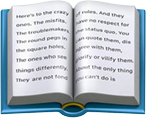
\includegraphics[height=7pt]{book emoji.png}\,{\scriptsize\color{gray!40!black}LLS}\par}}
\newcommand{\AFtag}{\par\vspace{2pt}{\raggedleft\scriptsize\itshape\color{ancfeuille}Anciennes feuilles\par}}
\newcommand{\VBlank}{\rule[0.15ex]{0.55cm}{0.35pt}}
\newcommand{\wallpapermotif}[1]{%
\begin{scope}[shift={#1}]
\fill[yellow!30!white,draw=gray!60,thick]
 (0,0.55) .. controls (0.35,0.75) and (0.55,0.35) .. (0.75,0)
 .. controls (0.55,-0.35) and (0.35,-0.75) .. (0,-0.55)
 .. controls (-0.35,-0.75) and (-0.55,-0.35) .. (-0.75,0)
 .. controls (-0.55,0.35) and (-0.35,0.75) .. (0,0.55) -- cycle;
\end{scope}}
\newcommand{\Jtag}{\par\vspace{2pt}{\raggedleft\scriptsize\itshape\color{jimmycolor}Fiches Jimmy\par}}
\newcommand{\Objectif}[1]{%
\vspace{16pt}
\noindent\begin{tcolorbox}[boxrule=1pt,colframe=black,colback=gray!7,arc=2pt,left=8pt,right=8pt,top=6pt,bottom=6pt]
\large\bfseries #1
\end{tcolorbox}
\vspace{8pt}
}
\newcommand{\ObjectifVide}{{\small\itshape\color{gray!45!black}Aucun exercice du manuel pour cet objectif pour l'instant (\`a compl\'eter avec les anciennes feuilles / fiches Jimmy).}\vspace{8pt}\par}
\title{\textbf{S\'equence 2 --- Banque des exercices}\\[4pt]\large Vecteurs}
\author{Manuel du Livre Scolaire p.~184 \`a 212 --- Lyc\'ee Lebrun Coutances}
\date{}
\begin{document}
\maketitle
\noindent Ce document reprend, en LaTeX, les exercices class\'es selon les 7 objectifs retenus pour la s\'equence~: exercices du manuel (\'etiquette bleue, tag \og LLS \fg), exercices des anciennes feuilles maison F4 \`a F6 (\'etiquette violette) et exercices des fiches Jimmy (\'etiquette orange). Seuls les exercices encadr\'es sont actifs~; les autres (retenus mais pas encore mis en forme/valid\'es) sont laiss\'es en commentaire dans le code source, \`a l'endroit o\`u ils devront figurer. Dans chaque objectif, les exercices sont tri\'es par difficult\'e croissante (pour l'Objectif 5~: d'abord le produit par un r\'eel, puis la colin\'earit\'e, chaque groupe tri\'e par difficult\'e).\\[3pt]
\noindent{\small Niveau de difficult\'e estim\'e~: \starfull{diffgreen}\starempty\starempty~facile \quad \starempty\starfull{diffblue}\starempty~moyen \quad \starempty\starempty\starfull{diffred}~difficile \textit{(appr\'eciation indicative, \`a ajuster).}}\\[3pt]
\noindent{\small\itshape\color{gray!45!black}Les figures sont des reproductions simplifi\'ees (sch\'ematiques) de celles du manuel, redessin\'ees en TikZ \`a partir des captures d'\'ecran~; elles ne sont pas pixel-\`a-pixel fid\`eles \`a l'original.}

\vspace{6pt}

\Objectif{Objectif 1 : Vecteur $\Vj{MM'}$ associ\'e \`a la translation qui transforme $M$ en $M'$ --- Direction, sens et norme}

\begin{tcolorbox}[boxrule=0.8pt,colframe=black,colback=white,arc=2pt,left=6pt,right=6pt,top=5pt,bottom=5pt]
\noindent{\bfseries\color{ancfeuille}\underline{F4 -- Exercice 2}}\ \starfull{diffgreen}\starempty\starempty\hfill{\color{gray!40!black}Repr\'esenter}\\
La figure ci-dessous repr\'esente sept hexagones r\'eguliers et num\'erot\'es.
\begin{center}
\begin{tikzpicture}[scale=0.28]
\draw (2,0)-- (4,0)-- (5,1.73)-- (4,3.46)-- (2,3.46)-- (1,1.73)-- cycle;
\draw (3,1.73) node[draw,circle]{1};
\draw (4,3.46)-- (5,5.2)-- (4,6.93)-- (2,6.93)-- (1,5.2)-- (2,3.46);
\draw (3,5.2) node[draw,circle]{2};
\draw (5,1.73) --(7,1.73)-- (8,3.46)-- (7,5.2)-- (5,5.2);
\draw (6,3.46) node[draw,circle]{3};
\draw (4,0)-- (5,-1.73)-- (7,-1.73)-- (8,0)--(7,1.73);
\draw (6,0) node[draw,circle]{4};
\draw (8,0)-- (10,0)-- (11,1.73)-- (10,3.46)-- (8,3.46);
\draw (9,1.73) node[draw,circle]{5};
\draw (10,3.46)-- (11,5.2)-- (10,6.93)-- (8,6.93)-- (7,5.2);
\draw (9,5.2) node[draw,circle]{6};
\draw (8,6.93)-- (7,8.66)-- (5,8.66)-- (4,6.93);
\draw (6,6.93) node[draw,circle]{7};
\draw (2,3.46) node[left] {$A$};
\draw (5,8.66) node[left] {$B$};
\draw (8,6.93) node[above right] {$C$};
\draw (11,5.2) node[right] {$D$};
\draw (11,1.73) node[right] {$E$};
\end{tikzpicture}
\end{center}
D\'eterminer l'image~:
\begin{enumerate}
\item de l'hexagone 1 dans la translation de vecteur $\Vj{AC}$~;
\item de l'hexagone 4 dans la translation de vecteur $\Vj{AB}$~;
\item de l'hexagone 7 dans la translation de vecteur $\Vj{DE}$.
\end{enumerate}
\AFtag
\end{tcolorbox}
\vspace{10pt}\par

\begin{tcolorbox}[boxrule=0.8pt,colframe=black,colback=white,arc=2pt,left=6pt,right=6pt,top=5pt,bottom=5pt]
\noindent{\bfseries\color{vecblue}\underline{Ex 28 p 185}}\ \starfull{diffgreen}\starempty\starempty\hfill{\color{gray!40!black}Communiquer}\\
On consid\`ere la figure suivante compos\'ee de triangles \'equilat\'eraux. Recopier et compl\'eter les phrases suivantes.
\begin{center}
\begin{tikzpicture}[scale=0.55]
\coordinate (Pa) at (0,0); \coordinate (Pi) at (5,0); \coordinate (Pe) at (2.5,4.33);
\begin{scope}
\clip (Pa) -- (Pi) -- (Pe) -- cycle;
\fill[teal!55] (Pa) -- (Pi) -- (Pe) -- cycle;
% horizontales (parall\`eles \`a la base)
\draw[white,thin] (0.625,1.0825) -- (4.375,1.0825);
\draw[white,thin] (1.25,2.165) -- (3.75,2.165);
\draw[white,thin] (1.875,3.2475) -- (3.125,3.2475);
% parall\`eles au c\^ot\'e gauche (base -> c\^ot\'e droit)
\draw[white,thin] (1.25,0) -- (3.125,3.2475);
\draw[white,thin] (2.5,0) -- (3.75,2.165);
\draw[white,thin] (3.75,0) -- (4.375,1.0825);
% parall\`eles au c\^ot\'e droit (base -> c\^ot\'e gauche)
\draw[white,thin] (3.75,0) -- (1.875,3.2475);
\draw[white,thin] (2.5,0) -- (1.25,2.165);
\draw[white,thin] (1.25,0) -- (0.625,1.0825);
\end{scope}
\draw[thick] (Pa) -- (Pi) -- (Pe) -- cycle;
\node[above] at (Pe) {$E$};
\node[above left] at (1.875,3.2475) {$D$}; \node[above right] at (3.125,3.2475) {$F$};
\node[left] at (1.25,2.165) {$C$}; \node[right] at (3.75,2.165) {$G$};
\node[left] at (0.625,1.0825) {$B$}; \node[right] at (4.375,1.0825) {$H$};
\node[below] at (0,0) {$A$}; \node[below] at (1.25,0) {$L$}; \node[below] at (2.5,0) {$K$}; \node[below] at (3.75,0) {$J$}; \node[below] at (5,0) {$I$};
\end{tikzpicture}
\end{center}
\begin{enumerate}
\item Le point $D$ a pour image le point \dots{} par la translation de vecteur $\Vj{G\dots}$.
\item $\dots=\dots$ signifie que \dots{} est l'image de \dots{} par la translation de vecteur \dots{}.
\end{enumerate}
\LLStag
\end{tcolorbox}
\vspace{10pt}\par

\begin{tcolorbox}[boxrule=0.8pt,colframe=black,colback=white,arc=2pt,left=6pt,right=6pt,top=5pt,bottom=5pt]
\noindent{\bfseries\color{vecblue}\underline{Ex 30 p 185}}\ \starfull{diffgreen}\starempty\starempty\hfill{\color{gray!40!black}Communiquer}\\
Voici les motifs d'un papier peint dont le pavage rappelle les \oe uvres de l'artiste Maurits Cornelis Escher (1898 -- 1972).
\begin{center}
{\small\itshape (motif de papier peint simplifi\'e~: pavage par translations, 10 motifs num\'erot\'es et 6 points de r\'ef\'erence $A$ \`a $F$)}\\[4pt]
\begin{tikzpicture}[scale=0.55]
\foreach \x in {0,1.8,3.6,5.4,7.2} \foreach \y in {0,1.8} \wallpapermotif{(\x,\y)}
\foreach \x/\n in {0/1,1.8/2,3.6/3,5.4/4,7.2/5}
 \node[circle,fill=black,text=white,inner sep=1.6pt,font=\scriptsize\bfseries] at (\x,2.2) {\n};
\foreach \x/\n in {0/6,1.8/7,3.6/8,5.4/9,7.2/10}
 \node[circle,fill=black,text=white,inner sep=1.6pt,font=\scriptsize\bfseries] at (\x,0.4) {\n};
\node[red,font=\bfseries\small] at (0.9,1.3) {$+\,A$};
\node[red,font=\bfseries\small] at (4.5,1.3) {$+\,B$};
\node[red,font=\bfseries\small] at (7.2,1.3) {$+\,C$};
\node[red,font=\bfseries\small] at (0.9,-0.5) {$+\,D$};
\node[red,font=\bfseries\small] at (4.5,-0.5) {$+\,E$};
\node[red,font=\bfseries\small] at (7.2,-0.5) {$+\,F$};
\end{tikzpicture}
\end{center}
\begin{enumerate}
\item \'Ecrire quatre phrases en utilisant l'expression \og est l'image de \fg. Par exemple~: \og La figure 8 est l'image de la figure 1 par la translation de vecteur $\Vj{AE}$. \fg
\item \'Ecrire quatre phrases en utilisant l'expression \og a pour image \fg.
\end{enumerate}
\LLStag
\end{tcolorbox}
\vspace{10pt}\par
\begin{tcolorbox}[boxrule=0.8pt,colframe=black,colback=white,arc=2pt,left=6pt,right=6pt,top=5pt,bottom=5pt]
\noindent{\bfseries\color{ancfeuille}\underline{F4 -- Exercice 1}}\ \starfull{diffgreen}\starempty\starempty\hfill{\color{gray!40!black}Repr\'esenter}\\
\`A partir de la figure ci-dessous,
\begin{enumerate}
\item donner les images des points $C$, $D$, $E$ dans la translation de vecteur $\Vj{AB}$~;
\item citer trois vecteurs \'egaux au vecteur $\Vj{AB}$~;
\item citer les trois parall\'elogrammes d\'efinis par les trois \'egalit\'es vectorielles pr\'ec\'edentes.
\end{enumerate}
\begin{center}
\begin{tikzpicture}[scale=0.5]
\draw[thin,gray!35] (-0.5,-0.5) grid (7.5,5.5);
\coordinate (A) at (1,4); \coordinate (B) at (4,5);
\coordinate (C) at (2,2); \coordinate (D) at (4,1); \coordinate (E) at (1,0);
\coordinate (Y) at (5,3); \coordinate (Z) at (7,2); \coordinate (X) at (6,1);
\draw[-{Stealth},thick] (A) -- (B);
\node[left] at (A) {$A$}; \node[above] at (B) {$B$};
\foreach \p in {C,D,E,Y,Z,X} \fill (\p) circle(1.5pt);
\node[left] at (C) {$C$}; \node[left] at (D) {$D$}; \node[above] at (E) {$E$};
\node[right] at (Y) {$Y$}; \node[left] at (Z) {$Z$}; \node[right] at (X) {$X$};
\end{tikzpicture}
\end{center}
\AFtag
\end{tcolorbox}
\vspace{10pt}\par

\begin{tcolorbox}[boxrule=0.8pt,colframe=black,colback=white,arc=2pt,left=6pt,right=6pt,top=5pt,bottom=5pt]
\noindent{\bfseries\color{vecblue}\underline{Ex 32 p 185}}\ \starempty\starfull{diffblue}\starempty\hfill{\color{gray!40!black}Repr\'esenter}\\
Reproduire la figure suivante sur papier point\'e.
\begin{center}
\begin{tikzpicture}[scale=0.6]
\foreach \x in {0,...,6} \foreach \y in {0,...,4} \fill[gray!60] (\x,\y) circle(0.7pt);
\coordinate (E) at (2,4); \coordinate (B) at (0,2); \coordinate (X) at (4,2); \coordinate (L) at (0,0);
\node[green!50!black,above] at (E) {$+E$}; \node[green!50!black,left] at (B) {$+B$};
\node[green!50!black,right] at (X) {$+X$}; \node[green!50!black,left] at (L) {$+L$};
\end{tikzpicture}
\end{center}
\begin{enumerate}
\item Construire les points $F$ et $A$, images de $E$ et $L$ par la translation de vecteur $\Vj{BX}$.
\item Construire les points $G$ et $H$, images de $E$ et $F$ par la translation de vecteur $\Vj{BL}$.
\item Tracer en traits pleins les segments $[BE]$, $[BX]$, $[BL]$, $[LA]$, $[XA]$, $[AH]$, $[FH]$, $[EF]$, $[XF]$ puis, en pointill\'es, les segments $[GE]$, $[GL]$ et $[GH]$.
\item Quel solide obtient-on~?
\end{enumerate}
\LLStag
\end{tcolorbox}
\vspace{10pt}\par

\Objectif{Objectif 2 : \'Egalit\'e de deux vecteurs, vecteur nul}

\begin{tcolorbox}[boxrule=0.8pt,colframe=black,colback=white,arc=2pt,left=6pt,right=6pt,top=5pt,bottom=5pt]
\noindent{\bfseries\color{vecblue}\underline{Ex 27 p 185}}\ \starfull{diffgreen}\starempty\starempty\hfill{\color{gray!40!black}Communiquer}\\
On consid\`ere les vecteurs suivants repr\'esent\'es sur un quadrillage.
\begin{center}
\begin{tikzpicture}[scale=0.55]
\draw[thin,cyan!30] (-0.5,0.5) grid (9.5,3.5);
\coordinate (M) at (0,3); \coordinate (A) at (1,3); \coordinate (B) at (3,3);
\coordinate (L) at (0,2); \coordinate (F) at (1,2); \coordinate (I) at (4,2);
\coordinate (G) at (0,1); \coordinate (H) at (5,1);
\draw[-{Stealth},thick] (A) -- (B);
\draw[-{Stealth},thick] (L) -- (M);
\draw[-{Stealth},thick] (F) -- (G);
\draw[-{Stealth},thick] (H) -- (I);
\node[left] at (M) {$M$}; \node[above] at (A) {$A$}; \node[above] at (B) {$B$};
\node[left] at (L) {$L$}; \node[above] at (F) {$F$}; \node[above left] at (I) {$I$};
\node[below] at (G) {$G$}; \node[below right] at (H) {$H$};
\fill (M) circle(1.3pt) (A) circle(1.3pt) (B) circle(1.3pt) (L) circle(1.3pt) (F) circle(1.3pt) (I) circle(1.3pt) (G) circle(1.3pt) (H) circle(1.3pt);
\coordinate (P1) at (7,2); \coordinate (P0) at (7,1);
\draw[-{Stealth},thick] (P1) -- (P0) node[midway,left]{$\vec p$};
\draw[-{Stealth},thick] (P0) -- (8.5,2) node[midway,above]{$\vec v$};
\draw[-{Stealth},thick] (8,1) -- (6,1) node[midway,below]{$\vec w$};
\draw[-{Stealth},thick] (7.3,1.5) -- (8.8,1.5) node[midway,above]{$\vec k$};
\draw[-{Stealth},thick] (8.7,3) -- (8.7,2) node[midway,right]{$\vec c$};
\end{tikzpicture}
\end{center}
\begin{enumerate}
\item Rep\'erer les vecteurs \'egaux, les vecteurs oppos\'es et les vecteurs de m\^eme norme.
\item Quelle est l'image du point $F$ par la translation de vecteur $\Vj{LM}$~?
\item Par quelles translations le point $A$ est-il l'image du point $B$~?
\end{enumerate}
\LLStag
\end{tcolorbox}
\vspace{10pt}\par

\begin{tcolorbox}[boxrule=0.8pt,colframe=black,colback=white,arc=2pt,left=6pt,right=6pt,top=5pt,bottom=5pt]
\noindent{\bfseries\color{jimmycolor}\underline{Exercice J1}}\ \starfull{diffgreen}\starempty\starempty\hfill{\color{gray!40!black}Chercher}\\
Citer les vecteurs repr\'esent\'es ci-contre~:
\begin{enumerate}
\item[a.] qui ont la m\^eme direction~;
\item[b.] qui ont la m\^eme direction et le m\^eme sens~;
\item[c.] qui ont la m\^eme norme.
\end{enumerate}
\begin{center}
\begin{tikzpicture}[scale=0.5]
\draw[thin,gray!35] (-0.5,-0.5) grid (7.5,5.5);
\coordinate (I) at (0,4); \coordinate (A) at (1,4); \coordinate (B) at (5,4);
\coordinate (J) at (0,1); \coordinate (D) at (1,3); \coordinate (C) at (4,3);
\coordinate (E) at (1,2); \coordinate (F) at (5,2.5);
\coordinate (G) at (7,0.5); \coordinate (H) at (4,0.3);
\draw[-{Stealth},thick,red] (A) -- (B); \node[left] at (I) {$I$}; \node[above] at (A) {$A$}; \node[above] at (B) {$B$};
\draw[-{Stealth},thick,orange] (I) -- (J); \node[below] at (J) {$J$};
\draw[-{Stealth},thick,blue] (D) -- (C); \node[left] at (D) {$D$}; \node[above] at (C) {$C$};
\draw[-{Stealth},thick,green!55!black] (E) -- (F); \node[left] at (E) {$E$}; \node[above] at (F) {$F$};
\draw[-{Stealth},thick,purple] (G) -- (H); \node[right] at (G) {$G$}; \node[below] at (H) {$H$};
\end{tikzpicture}
\end{center}
\Jtag
\end{tcolorbox}
\vspace{10pt}\par

\begin{tcolorbox}[boxrule=0.8pt,colframe=black,colback=white,arc=2pt,left=6pt,right=6pt,top=5pt,bottom=5pt]
\noindent{\bfseries\color{jimmycolor}\underline{Exercice J4}}\ \starfull{diffgreen}\starempty\starempty\hfill{\color{gray!40!black}Calculer}\\
$EFGH$ est un parall\'elogramme de centre $I$ repr\'esent\'e ci-contre.
\begin{center}
\begin{tikzpicture}[scale=0.9]
\coordinate (E) at (0,1.3); \coordinate (F) at (3,1.5); \coordinate (H) at (0.5,0); \coordinate (G) at (3.3,0.2);
\coordinate (I) at ($(E)!0.5!(G)$);
\draw[thick,teal!45] (E) -- (F) -- (G) -- (H) -- cycle; \draw[thick,teal!45] (E) -- (G); \draw[thick,teal!45] (F) -- (H);
\node[above] at (E) {$E$}; \node[above] at (F) {$F$}; \node[below] at (H) {$H$}; \node[below] at (G) {$G$}; \node[above] at (I) {$I$};
\end{tikzpicture}
\end{center}
\begin{enumerate}
\item Donner un vecteur \'egal \`a~: a. $\Vj{EF}$ \quad b. $\Vj{GH}$ \quad c. $\Vj{EH}$ \quad d. $\Vj{GF}$
\item Compl\'eter par le point qui convient~: a. $\Vj{EI}=\Vj{I\dots}$ \quad b. $\Vj{HI}=\Vj{I\dots}$ \quad c. $\Vj{FI}=\Vj{I\dots}$
\item[3.] a. Quel est le repr\'esentant d'origine $F$ du vecteur $\Vj{EH}$~?\\
b. Quel est le repr\'esentant d'origine $F$ du vecteur $\Vj{IH}$~?
\end{enumerate}
\Jtag
\end{tcolorbox}
\vspace{10pt}\par

\begin{tcolorbox}[boxrule=0.8pt,colframe=black,colback=white,arc=2pt,left=6pt,right=6pt,top=5pt,bottom=5pt]
\noindent{\bfseries\color{ancfeuille}\underline{F4 -- Exercice 4}}\ \starfull{diffgreen}\starempty\starempty\hfill{\color{gray!40!black}Raisonner}\\
Sur la figure suivante, expliquer, en utilisant les termes direction, sens ou norme, pourquoi le vecteur $\Vj{AB}$ n'est \'egal \`a aucun des autres vecteurs repr\'esent\'es.
\begin{center}
\begin{tikzpicture}[scale=0.6]
\foreach \x in {0,...,7} \foreach \y in {0,...,4} \fill[gray!55] (\x,\y) circle(0.6pt);
\draw[-{Stealth},thick] (0,2) -- (1,3); \node[below] at (0,2) {$A$}; \node[above] at (1,3) {$B$};
\draw[-{Stealth},thick] (1,0) -- (3,0); \node[below] at (1,0) {$C$}; \node[below] at (3,0) {$D$};
\draw[-{Stealth},thick] (3,2) -- (5,4); \node[below] at (3,2) {$G$}; \node[above] at (5,4) {$H$};
\draw[-{Stealth},thick] (7,2) -- (6,1); \node[below] at (6,1) {$E$}; \node[above] at (7,2) {$F$};
\end{tikzpicture}
\end{center}
\AFtag
\end{tcolorbox}
\vspace{10pt}\par

\begin{tcolorbox}[boxrule=0.8pt,colframe=black,colback=white,arc=2pt,left=6pt,right=6pt,top=5pt,bottom=5pt]
\noindent{\bfseries\color{vecblue}\underline{Ex 23 p 184}}\ \starfull{diffgreen}\starempty\starempty\hfill{\color{gray!40!black}Raisonner}\\
Un enseignant est en train de corriger une copie d'un de ses \'el\`eves.
\begin{center}
\begin{minipage}{0.8\linewidth}
\itshape\ttfamily\small
Deux vecteurs \'egaux sont confondus.\\
Si $I$ est milieu alors $\Vj{AI}=\Vj{BI}$.\\
Si $I$ appartient \`a la m\'ediatrice de $[AB]$ alors $\Vj{AI}=\Vj{IB}$.
\end{minipage}
\end{center}
Ces phrases sont-elles correctes~? Justifier la r\'eponse.
\LLStag
\end{tcolorbox}
\vspace{10pt}\par

\begin{tcolorbox}[boxrule=0.8pt,colframe=black,colback=white,arc=2pt,left=6pt,right=6pt,top=5pt,bottom=5pt]
\noindent{\bfseries\color{ancfeuille}\underline{F4 -- Exercice 3}}\ \starempty\starfull{diffblue}\starempty\hfill{\color{gray!40!black}Repr\'esenter}\\
\`A partir de la figure ci-dessous, citer un vecteur~:
\begin{enumerate}
\item oppos\'e \`a $\Vj{CD}$~;
\item de m\^eme direction et de m\^eme sens que $\Vj{AC}$~;
\item de m\^eme direction que $\Vj{BC}$ mais de sens contraire~;
\item \'egal au vecteur $\Vj{BA}$.
\end{enumerate}
\begin{center}
\begin{tikzpicture}[scale=0.45]
\draw[thin,gray!35] (-0.5,-0.5) grid (9.5,8.5);
\coordinate (A) at (3,4); \coordinate (B) at (1,1); \coordinate (C) at (3,1); \coordinate (D) at (4,2);
\foreach \p in {A,B,C,D} \fill (\p) circle(1.5pt);
\node[left] at (A) {$A$}; \node[below] at (B) {$B$}; \node[below] at (C) {$C$}; \node[below] at (D) {$D$};
\draw[-{Stealth},thick] (0,3) -- (1,3) node[midway,above]{$\vec u$};
\draw[-{Stealth},thick] (1,5) -- (3,8) node[midway,above left]{$\vec v$};
\draw[-{Stealth},thick] (4,5) -- (4,7) node[midway,left]{$\vec w$};
\draw[-{Stealth},thick] (5,6) -- (6,7) node[midway,above]{$\vec r$};
\draw[-{Stealth},thick] (8,8) -- (6,3) node[midway,above]{$\vec s$};
\draw[-{Stealth},thick] (8,8) -- (7,8) node[midway,above]{$\vec t$};
\draw[-{Stealth},thick] (9,2) -- (8,1) node[midway,above]{$\vec p$};
\draw[-{Stealth},thick] (9,5) -- (9,4) node[midway,left]{$\vec m$};
\end{tikzpicture}
\end{center}
\AFtag
\end{tcolorbox}
\vspace{10pt}\par

\begin{tcolorbox}[boxrule=0.8pt,colframe=black,colback=white,arc=2pt,left=6pt,right=6pt,top=5pt,bottom=5pt]
\noindent{\bfseries\color{vecblue}\underline{Ex 29 p 185}}\ \starempty\starfull{diffblue}\starempty\hfill{\color{gray!40!black}Communiquer}\\
On consid\`ere un parall\'elogramme $ABCD$ de centre $O$ et le triangle \'equilat\'eral $BCE$. $G$, $H$ et $I$ sont les milieux respectifs de $[BE]$, de $[CE]$ et de $[BC]$.
\begin{enumerate}
\item Faire une figure \`a main lev\'ee.
\item Indiquer trois couples de vecteurs \'egaux deux \`a deux en justifiant \`a l'aide de propri\'et\'es vectorielles du cours.
\end{enumerate}
\LLStag
\end{tcolorbox}
\vspace{10pt}\par

\begin{tcolorbox}[boxrule=0.8pt,colframe=black,colback=white,arc=2pt,left=6pt,right=6pt,top=5pt,bottom=5pt]
\noindent{\bfseries\color{jimmycolor}\underline{Exercice J2}}\ \starempty\starfull{diffblue}\starempty\hfill{\color{gray!40!black}Chercher}\\
$\vec u$ est un vecteur donn\'e. Repasser en couleur le(s) vecteur(s) \'egal (\'egaux) \`a $\vec u$. Un de ces vecteurs est l'oppos\'e du vecteur $\vec u$~: essayer de d\'eterminer lequel et tenter de d\'efinir la notion de vecteurs oppos\'es.
\begin{center}
{\small\itshape (figure simplifi\'ee~: $\vec u$ et huit vecteurs candidats A-A' \`a H-H' de directions/longueurs vari\'ees)}\\[4pt]
\begin{tikzpicture}[scale=0.55]
\draw[-{Stealth},thick] (0,0) -- (2,1); \node[below] at (0.5,0.2) {$\vec u$};
\draw[-{Stealth},thick] (4,7) -- (5.5,7.7); \node[left] at (4,7) {$A$}; \node[right] at (5.5,7.7) {$A'$};
\draw[-{Stealth},thick] (4,6) -- (5.5,6.4); \node[left] at (4,6) {$B$}; \node[right] at (5.5,6.4) {$B'$};
\draw[-{Stealth},thick] (4,5) -- (5,4.3); \node[left] at (4,5) {$C$}; \node[right] at (5,4.3) {$C'$};
\draw[-{Stealth},thick] (4,3.7) -- (5.8,4.3); \node[left] at (4,3.7) {$D$}; \node[right] at (5.8,4.3) {$D'$};
\draw[-{Stealth},thick] (4,2.7) -- (5.7,3.3); \node[left] at (4,2.7) {$E$}; \node[right] at (5.7,3.3) {$E'$};
\draw[-{Stealth},thick] (4,1.7) -- (5.2,1.3); \node[left] at (4,1.7) {$F$}; \node[right] at (5.2,1.3) {$F'$};
\draw[-{Stealth},thick] (5.5,0.5) -- (4,0); \node[right] at (5.5,0.5) {$G$}; \node[left] at (4,0) {$G'$};
\draw[-{Stealth},thick] (4,-1) -- (5.5,-0.3); \node[left] at (4,-1) {$H$}; \node[right] at (5.5,-0.3) {$H'$};
\end{tikzpicture}
\end{center}
\Jtag
\end{tcolorbox}
\vspace{10pt}\par

\begin{tcolorbox}[boxrule=0.8pt,colframe=black,colback=white,arc=2pt,left=6pt,right=6pt,top=5pt,bottom=5pt]
\noindent{\bfseries\color{jimmycolor}\underline{Exercice J3}}\ \starempty\starfull{diffblue}\starempty\hfill{\color{gray!40!black}Chercher}\\
Retrouver les vecteurs \'egaux dans la figure~:
\begin{center}
\begin{tikzpicture}[scale=0.7]
\coordinate (A) at (0,3); \coordinate (B) at (2,3); \coordinate (C) at (4,3);
\coordinate (E) at (0,1.5); \coordinate (D) at (3,2); \coordinate (G) at (4,1.5);
\coordinate (H) at (1.5,0.7); \coordinate (F) at (2,0); \coordinate (I) at (0,0); \coordinate (J) at (2,0); \coordinate (K) at (4,0);
\draw[thick] (A) -- (C); \draw[thick] (E) -- (G); \draw[thick] (I) -- (K);
\draw[thick] (A) -- (K); \draw[thick] (A) -- (J); \draw[thick] (E) -- (C); \draw[thick] (I) -- (D);
\node[above] at (A) {$A$}; \node[above] at (B) {$B$}; \node[above] at (C) {$C$};
\node[left] at (E) {$E$}; \node[above] at (D) {$D$}; \node[right] at (G) {$G$};
\node[below] at (H) {$H$}; \node[below] at (I) {$I$}; \node[below] at (J) {$J$}; \node[below] at (K) {$K$};
\end{tikzpicture}
\end{center}
\begin{center}
{\scriptsize
\begin{tabular}{|l|}
\hline
$\Vj{AB}=\dots=\dots=\dots=\dots=\dots$\\
\hline
$\Vj{FK}=\dots=\dots=\dots$\\
\hline
$\Vj{CD}=\dots=\dots=\dots$\\
\hline
$\Vj{IE}=\dots=\dots=\dots$\\
\hline
$\Vj{HC}=\dots$\\
\hline
\end{tabular}}
\end{center}
\Jtag
\end{tcolorbox}
\vspace{10pt}\par

\begin{tcolorbox}[boxrule=0.8pt,colframe=black,colback=white,arc=2pt,left=6pt,right=6pt,top=5pt,bottom=5pt]
\noindent{\bfseries\color{vecblue}\underline{Ex 18 p 183}}\ \starempty\starfull{diffblue}\starempty\hfill{\color{gray!40!black}Raisonner}\\
Voici des extraits de copies d'\'el\`eves r\'ecup\'er\'es par un professeur. \`A l'aide d'un sch\'ema, d'une d\'efinition ou d'un contre-exemple, relever et expliquer les erreurs en justifiant.
\begin{center}
\begin{minipage}{0.85\linewidth}
\itshape\ttfamily\small
$\bullet$ L'oppos\'e du vecteur $\Vj{AE}$ est $\overleftarrow{\text{AE}}$.\\[4pt]
$\bullet$ Si $ABCD$ est un parall\'elogramme alors $\Vj{AC}=\Vj{BD}$.\\[4pt]
$\bullet$ Si $\Vj{AB}=\Vj{CD}$ alors $ABCD$ est un parall\'elogramme.\\[4pt]
$\bullet$ Si $\Vj{AC}=\Vj{BD}$ alors $[AB]$ et $[CD]$ ont le m\^eme milieu.
\end{minipage}
\end{center}
\LLStag
\end{tcolorbox}
\vspace{10pt}\par
\begin{tcolorbox}[boxrule=0.8pt,colframe=black,colback=white,arc=2pt,left=6pt,right=6pt,top=5pt,bottom=5pt]
\noindent{\bfseries\color{jimmycolor}\underline{Exercice J7}}\ \starempty\starfull{diffblue}\starempty\hfill{\color{gray!40!black}Raisonner}\\
Soient $ABCD$ et $ABEF$ deux parall\'elogrammes.
\begin{center}
\begin{tikzpicture}[scale=0.8]
\coordinate (A) at (0,0); \coordinate (B) at (2.2,0); \coordinate (D) at (0.6,1.5); \coordinate (C) at (2.8,1.5);
\coordinate (F) at (0.9,2.2); \coordinate (E) at (3.1,2.2);
\draw[green!45!black] (A)--(B)--(C)--(D)--cycle;
\draw[teal] (A)--(B)--(E)--(F)--cycle;
\node[below] at (A) {$A$}; \node[below] at (B) {$B$}; \node[left] at (D) {$D$}; \node[right] at (C) {$C$};
\node[left] at (F) {$F$}; \node[right] at (E) {$E$};
\end{tikzpicture}
\end{center}
\begin{enumerate}
\item Donner deux vecteurs \'egaux au vecteur $\Vj{AB}$.
\item En d\'eduire la nature du quadrilat\`ere $EFDC$.
\end{enumerate}
\Jtag
\end{tcolorbox}
\vspace{10pt}\par

\begin{tcolorbox}[boxrule=0.8pt,colframe=black,colback=white,arc=2pt,left=6pt,right=6pt,top=5pt,bottom=5pt]
\noindent{\bfseries\color{jimmycolor}\underline{Exercice J8}}\ \starempty\starfull{diffblue}\starempty\hfill{\color{gray!40!black}Raisonner}\\
Sur la figure ci-contre, $ABCD$ est un rectangle, et $AEBC$ et $ACDF$ sont des parall\'elogrammes.
\begin{center}
\begin{tikzpicture}[scale=0.8]
\coordinate (D) at (0,2); \coordinate (C) at (3,2); \coordinate (A) at (0,0); \coordinate (B) at (3,0);
\coordinate (F) at (-1.8,1); \coordinate (E) at (0,-1.8);
\draw[blue] (D)--(C)--(B)--(A)--cycle;
\draw[green!50!black] (F)--(A)--(C)--(D)--cycle;
\draw[red] (F)--(A)--(E)--(B);
\node[above] at (D) {$D$}; \node[above] at (C) {$C$}; \node[below] at (A) {$A$}; \node[below] at (B) {$B$};
\node[left] at (F) {$F$}; \node[below] at (E) {$E$};
\end{tikzpicture}
\end{center}
\begin{enumerate}
\item Montrer que $\Vj{EB}=\Vj{FD}$.
\item Montrer que le quadrilat\`ere $EBDF$ est un parall\'elogramme de centre $A$.
\end{enumerate}
\Jtag
\end{tcolorbox}
\vspace{10pt}\par

\begin{tcolorbox}[boxrule=0.8pt,colframe=black,colback=white,arc=2pt,left=6pt,right=6pt,top=5pt,bottom=5pt]
\noindent{\bfseries\color{jimmycolor}\underline{Exercice J5}}\ \starempty\starempty\starfull{diffred}\hfill{\color{gray!40!black}Chercher}\\
La figure ci-contre repr\'esente six parall\'elogrammes identiques.
\begin{center}
\begin{tikzpicture}[scale=0.7]
\foreach \x/\lab in {0/A,1/B,2/C,3/D} \coordinate (\lab) at (\x+1,2);
\foreach \x/\lab in {0/H,1/G,2/F,3/E} \coordinate (\lab) at (\x+0.5,1);
\foreach \x/\lab in {0/I,1/J,2/K,3/L} \coordinate (\lab) at (\x,0);
\draw[red] (A) -- (D); \draw[red] (H) -- (E); \draw[red] (I) -- (L);
\draw[red] (A) -- (I); \draw[red] (B) -- (J); \draw[red] (C) -- (K); \draw[red] (D) -- (L);
\foreach \p in {A,B,C,D,H,G,F,E,I,J,K,L} \fill (\p) circle(1.2pt);
\node[above] at (A) {$A$}; \node[above] at (B) {$B$}; \node[above] at (C) {$C$}; \node[above] at (D) {$D$};
\node[left] at (H) {$H$}; \node[above] at (G) {$G$}; \node[above] at (F) {$F$}; \node[right] at (E) {$E$};
\node[below] at (I) {$I$}; \node[below] at (J) {$J$}; \node[below] at (K) {$K$}; \node[below] at (L) {$L$};
\end{tikzpicture}
\end{center}
\begin{enumerate}
\item[1.] a. Citer un vecteur qui a la m\^eme direction que le vecteur $\Vj{FG}$ mais pas le m\^eme sens et pas la m\^eme norme.\\
b. Citer un vecteur qui a la m\^eme direction que le vecteur $\Vj{EL}$, la m\^eme norme mais pas le m\^eme sens.
\item[2.] a. Citer le repr\'esentant d'origine $I$ du vecteur $\Vj{ED}$.\\
b. Citer le repr\'esentant d'origine $G$ du vecteur $\Vj{IK}$.
\item[3.] Citer un vecteur \'egal au vecteur $\Vj{HF}$.
\item[4.] a. Citer un vecteur oppos\'e au vecteur $\Vj{AB}$.\\
b. Citer le vecteur oppos\'e au vecteur $\Vj{CK}$ d'origine $J$.
\item[5.] a. Quelle est l'image du point $A$ par la translation de vecteur $\Vj{GF}$~?\\
b. Quelle est l'image du point $H$ par la translation de vecteur $\Vj{CE}$~?
\item[6.] a. Quel point a pour image $K$ par la translation de vecteur $\Vj{AI}$~?\\
b. Quel point a pour image $L$ par la translation de vecteur $\Vj{BE}$~?
\end{enumerate}
\Jtag
\end{tcolorbox}
\vspace{10pt}\par
\begin{tcolorbox}[boxrule=0.8pt,colframe=black,colback=white,arc=2pt,left=6pt,right=6pt,top=5pt,bottom=5pt]
\noindent{\bfseries\color{jimmycolor}\underline{Exercice J23} (pour aller plus loin)}\ \starempty\starempty\starfull{diffred}\hfill{\color{gray!40!black}Raisonner}\\
Sur la figure ci-contre, $ABCD$ est un parall\'elogramme, et $E$ et $F$ sont les points d\'efinis par~: $\Vj{AE}=\dfrac14\Vj{AB}$ et $\Vj{DF}=\dfrac34\Vj{DC}$.
\begin{center}
\begin{tikzpicture}[scale=0.9]
\coordinate (A) at (0,0); \coordinate (B) at (3,0); \coordinate (D) at (0.7,1.5); \coordinate (C) at (3.7,1.5);
\coordinate (E) at ($(A)!0.25!(B)$); \coordinate (F) at ($(D)!0.75!(C)$);
\draw[green!45!black] (A)--(B)--(C)--(D)--cycle;
\draw[red] (E)--(F);
\node[below] at (A) {$A$}; \node[below] at (B) {$B$}; \node[above] at (D) {$D$}; \node[above] at (C) {$C$};
\node[below] at (E) {$E$}; \node[above] at (F) {$F$};
\end{tikzpicture}
\end{center}
Montrer que le quadrilat\`ere $AECF$ est un parall\'elogramme.
\Jtag
\end{tcolorbox}

\Objectif{Objectif 3 : Repr\'esentants d'un vecteur}

\begin{tcolorbox}[boxrule=0.8pt,colframe=black,colback=white,arc=2pt,left=6pt,right=6pt,top=5pt,bottom=5pt]
\noindent{\bfseries\color{vecblue}\underline{Ex 31 p 185}}\ \starempty\starfull{diffblue}\starempty\hfill{\color{gray!40!black}Repr\'esenter}\\
On consid\`ere les vecteurs $\Vj{AB}$ et $\Vj{EF}$ et un point $C$.
\begin{center}
\begin{tikzpicture}[scale=0.55]
\draw[thin,cyan!30] (0,0) grid (8,5);
\coordinate (C) at (2,4); \coordinate (A) at (6,4); \coordinate (B) at (5,3);
\coordinate (E) at (5,1); \coordinate (F) at (3,1);
\draw[-{Stealth},thick] (A) -- (B) node[midway,left]{$\Vj{AB}$};
\draw[-{Stealth},thick] (E) -- (F) node[midway,above]{$\Vj{EF}$};
\node[above] at (C) {$+\,C$}; \node[above] at (A) {$+\,A$};
\node[below] at (B) {$B$}; \node[below] at (E) {$E$}; \node[below] at (F) {$F$};
\fill (C) circle(1.3pt) (A) circle(1.3pt) (E) circle(1.3pt);
\end{tikzpicture}
\end{center}
\begin{enumerate}
\item Reproduire la figure sur papier quadrill\'e.
\item Construire les points manquants.
\begin{enumerate}
\item[a.] $D$ tel que $\Vj{CD}=\Vj{AB}$
\item[b.] $G$ tel que $\Vj{CG}=\Vj{EF}$
\item[c.] $H$ tel que $\Vj{HC}=\Vj{AB}$
\item[d.] $I$ tel que $\Vj{IC}=\Vj{CG}$
\item[e.] $J$ tel que $\Vj{BJ}=\Vj{JC}$
\end{enumerate}
\end{enumerate}
\LLStag
\end{tcolorbox}
\vspace{10pt}\par

\Objectif{Objectif 4 : Somme de deux vecteurs et relation de Chasles}

\begin{tcolorbox}[boxrule=0.8pt,colframe=black,colback=white,arc=2pt,left=6pt,right=6pt,top=5pt,bottom=5pt]
\noindent{\bfseries\color{vecblue}\underline{Ex 39 p 186}}\ \starfull{diffgreen}\starempty\starempty\hfill{\color{gray!40!black}Repr\'esenter}\\
On consid\`ere les vecteurs suivants repr\'esent\'es sur du papier quadrill\'e.
\begin{center}
{\small\itshape (figure simplifi\'ee)}\\[4pt]
\begin{tikzpicture}[scale=0.55]
\coordinate (A) at (0,3); \coordinate (B) at (1,3.6); \coordinate (C) at (3,3.4);
\coordinate (L) at (1,1.3); \coordinate (D) at (2.4,1.3);
\draw[-{Stealth},thick] (A) -- (B); \draw[-{Stealth},thick] (A) -- (L);
\draw[-{Stealth},thick] (A) -- (D); \draw[-{Stealth},thick] (B) -- (C);
\draw[-{Stealth},thick] (C) -- (D); \draw[-{Stealth},thick] (L) -- (D);
\node[above] at (B) {$B$}; \node[above] at (C) {$C$}; \node[left] at (A) {$A$};
\node[below] at (L) {$L$}; \node[below] at (D) {$D$};
\coordinate (H) at (6.5,0.9); \coordinate (F) at (6.5,3.3);
\coordinate (Gp) at (4.5,0.2); \coordinate (Hc) at (5,1);
\draw[-{Stealth},thick] (Hc) -- ++(-1.2,0.1) node[midway,above]{$\vec c$};
\draw[-{Stealth},thick] (Hc) -- ++(0.8,0.9) node[midway,above]{$\vec b$};
\draw[-{Stealth},thick] (Hc) -- ++(1.1,0.4) node[midway,above]{$\vec k$};
\draw[-{Stealth},thick] (Hc) -- ++(0.9,1.2) node[midway,above]{$\vec d$};
\draw[-{Stealth},thick] ($(Hc)+(1.1,0.4)$) -- ++(0.3,0.9) node[midway,right]{$\vec r$};
\draw[-{Stealth},thick] (Gp) -- ++(0.5,0.7) node[midway,left]{$\vec f$};
\draw[-{Stealth},thick] (F) -- (H) node[midway,right]{};
\node[right] at (F) {$E$}; \node[right] at (H) {$F$};
\node[below] at (Gp) {$G$}; \node[left] at (Hc) {$H$};
\end{tikzpicture}
\end{center}
\begin{enumerate}
\item \'Ecrire cinq sommes de vecteurs traduisant la relation de Chasles.
\item Transformer les expressions suivantes de fa\c con \`a faire appara\^itre la relation de Chasles et \`a d\'eterminer le vecteur somme.
\begin{multicols}{2}
\begin{enumerate}
\item[a.] $\Vj{BC}+\Vj{EF}$
\item[b.] $\Vj{EF}+\Vj{LC}$
\item[c.] $\Vj{GH}+\Vj{BC}$
\item[d.] $\Vj{BC}+\vec b$
\end{enumerate}
\end{multicols}
\end{enumerate}
\LLStag
\end{tcolorbox}
\vspace{10pt}\par

\begin{tcolorbox}[boxrule=0.8pt,colframe=black,colback=white,arc=2pt,left=6pt,right=6pt,top=5pt,bottom=5pt]
\noindent{\bfseries\color{vecblue}\underline{Ex 42 p 187}}\ \starfull{diffgreen}\starempty\starempty\hfill{\color{gray!40!black}Repr\'esenter}\\
On consid\`ere les figures suivantes.
\begin{center}
\begin{tikzpicture}[scale=0.6]
\draw[thin,gray!35] (-0.5,0.5) grid (4,3.5);
\coordinate (M) at (0,3); \coordinate (C) at (1,3); \coordinate (B) at (0,1); \coordinate (A) at (2,1);
\draw[-{Stealth},thick] (B) -- (A) node[midway,below]{$\vec w$};
\draw[-{Stealth},thick] (2.3,2) -- ++(0.9,0.5) node[midway,above]{$\vec a$};
\node[above] at (M) {$M$}; \node[above] at (C) {$C$}; \node[below] at (B) {$B$}; \node[below] at (A) {$A$};
\fill (M) circle(1.3pt) (C) circle(1.3pt);
\end{tikzpicture}
\hspace{1cm}
\begin{tikzpicture}[scale=0.6]
\coordinate (J) at (2.3,3); \coordinate (L) at (3.6,2.7); \coordinate (K) at (3,1.3); \coordinate (N) at (2,0.4);
\draw[-{Stealth},thick] (K) -- ++(-0.7,0.9) node[midway,left]{$\vec b$};
\draw[-{Stealth},thick] (K) -- ++(0.7,0.9) node[midway,right]{$\vec c$};
\node[above] at (J) {$J$}; \node[right] at (L) {$L$}; \node[below] at (N) {$N$};
\fill (J) circle(1.3pt) (L) circle(1.3pt) (N) circle(1.3pt);
\end{tikzpicture}
\end{center}
\begin{enumerate}
\item Reproduire les figures.
\item Tracer les vecteurs~: $\Vj{AB}+\Vj{BC}$, $\vec w+\vec a$, $\vec b+\vec c$, $\Vj{JK}+\Vj{KL}$.
\item Placer les points $P$, $R$, $S$ et $T$ tels que~:
\begin{enumerate}
\item[a.] $\Vj{MR}$ soit \'egal au vecteur $\vec w+\vec a$.
\item[b.] $\Vj{NS}$ soit \'egal au vecteur somme $\vec b+\vec c$.
\item[c.] $\Vj{NT}$ soit \'egal au vecteur somme $\Vj{JK}+\Vj{KL}$.
\end{enumerate}
\end{enumerate}
\LLStag
\end{tcolorbox}
\vspace{10pt}\par

\begin{tcolorbox}[boxrule=0.8pt,colframe=black,colback=white,arc=2pt,left=6pt,right=6pt,top=5pt,bottom=5pt]
\noindent{\bfseries\color{jimmycolor}\underline{Exercice J11}}\ \starfull{diffgreen}\starempty\starempty\hfill{\color{gray!40!black}Repr\'esenter}\\
Reproduire la figure ci-contre, et construire les points $E$ et $F$ d\'efinis par~:
\begin{enumerate}
\item[a.] $\Vj{AE}=\vec u+\vec w$
\item[b.] $\Vj{BF}=2\vec v+\vec u$
\end{enumerate}
\begin{center}
\begin{tikzpicture}[scale=0.55]
\draw[thin,gray!35] (-4,-1) grid (5,4);
\coordinate (A) at (0,1);
\draw[-{Stealth},thick,green!55!black] (A) -- (-3,3) node[midway,above]{$\vec u$};
\draw[-{Stealth},thick,cyan!70!black] (A) -- (1.5,1) node[midway,above]{$\vec w$};
\draw[-{Stealth},thick,red] (4,3) -- (2,0.5) node[midway,right]{$\vec v$};
\node[below] at (A) {$A$}; \node[above right] at (4,3) {$B$};
\fill (A) circle(1.3pt) (4,3) circle(1.3pt);
\end{tikzpicture}
\end{center}
\Jtag
\end{tcolorbox}
\vspace{10pt}\par

\begin{tcolorbox}[boxrule=0.8pt,colframe=black,colback=white,arc=2pt,left=6pt,right=6pt,top=5pt,bottom=5pt]
\noindent{\bfseries\color{jimmycolor}\underline{Exercice J13}}\ \starfull{diffgreen}\starempty\starempty\hfill{\color{gray!40!black}Repr\'esenter}\\
Reproduire la figure ci-contre, et construire~:
\begin{enumerate}
\item[a.] Le point $E$ tel que $\Vj{AE}=\Vj{AB}+\Vj{AD}$.
\item[b.] Les points $F$ et $G$ tels que~: $\Vj{AF}=\Vj{CA}+\Vj{BA}$ et $\Vj{AG}=\Vj{AD}-\Vj{AC}$
\end{enumerate}
\begin{center}
\begin{tikzpicture}[scale=0.7]
\draw[thin,gray!35] (-0.5,-0.5) grid (4.5,3.5);
\coordinate (A) at (0,3); \coordinate (D) at (4,3); \coordinate (C) at (0,1); \coordinate (B) at (2,0);
\draw[-{Stealth},thick] (A) -- (D); \draw[-{Stealth},thick] (A) -- (B);
\node[above] at (A) {$A$}; \node[above] at (D) {$D$}; \node[left] at (C) {$C$}; \node[below] at (B) {$B$};
\fill (C) circle(1.3pt);
\end{tikzpicture}
\end{center}
\Jtag
\end{tcolorbox}
\vspace{10pt}\par

\iffalse
\noindent{\bfseries\color{vecblue}\underline{Ex 58 p 210}}\ \starfull{diffgreen}\starempty\starempty\hfill{\color{gray!40!black}Calculer}\\
Recopier et compl\'eter les \'egalit\'es suivantes.
\begin{enumerate}
\item $3\Vj{BC}+3\Vj{CD}=3(\dots+\dots)=\dots$
\item $5\Vj{MP}-3\Vj{MS}=5(\dots{}\Vj{R}+\dots)-3(\dots+\Vj{K}\dots)$
\end{enumerate}
\LLStag
\vspace{12pt}\par
\fi

\iffalse
\noindent{\bfseries\color{vecblue}\underline{Ex 59 p 210}}\ \starfull{diffgreen}\starempty\starempty\hfill{\color{gray!40!black}Calculer}\\
Simplifier les expressions suivantes sous la forme d'une somme de deux vecteurs.
\begin{enumerate}
\item $\Vj{MC}+2\Vj{KL}+2\Vj{LS}-\Vj{TC}$
\item $\Vj{KL}+3\Vj{LM}-2\Vj{RM}$
\end{enumerate}
\LLStag
\vspace{12pt}\par
\fi

\begin{tcolorbox}[boxrule=0.8pt,colframe=black,colback=white,arc=2pt,left=6pt,right=6pt,top=5pt,bottom=5pt]
\noindent{\bfseries\color{jimmycolor}\underline{Exercice J19}}\ \starfull{diffgreen}\starempty\starempty\hfill{\color{gray!40!black}Mod\'eliser}\\
Un solide est soumis \`a trois forces $\vec{F_1}$, $\vec{F_2}$ et $\vec{F_3}$. Reproduire la figure et construire, en choisissant comme origine le point $G$, le vecteur $\vec{F_1}+\vec{F_2}+\vec{F_3}$.
\begin{center}
\begin{tikzpicture}[scale=0.6]
\draw[thin,gray!35] (-2,-2) grid (2,2);
\coordinate (G) at (0,0);
\draw[-{Stealth},thick,red] (G) -- (1.5,1.5) node[midway,above]{$\vec{F_1}$};
\draw[-{Stealth},thick,red] (G) -- (0,-1.5) node[midway,left]{$\vec{F_2}$};
\draw[-{Stealth},thick,red] (G) -- (-1.5,0.5) node[midway,above]{$\vec{F_3}$};
\node[below right] at (G) {$G$};
\end{tikzpicture}
\end{center}
\Jtag
\end{tcolorbox}
\vspace{10pt}\par

\begin{tcolorbox}[boxrule=0.8pt,colframe=black,colback=white,arc=2pt,left=6pt,right=6pt,top=5pt,bottom=5pt]
\noindent{\bfseries\color{vecblue}\underline{Ex 69 p 191}}\ \starfull{diffgreen}\starempty\starempty\hfill{\color{gray!40!black}Repr\'esenter}\\
Une p\'eniche est tir\'ee par deux personnes \`a l'aide de cordes sur le chemin de halage qui longe le canal. Les vecteurs d\'ecrivent les deux forces en termes de sens, de direction et d'intensit\'e.
\begin{center}
\begin{tikzpicture}[scale=0.5]
\fill[green!25] (-6,-2.6) rectangle (6,2.6);
\fill[cyan!12] (-6,-1.6) rectangle (6,1.6);
\draw[brown!60!orange,thick] (-6,-1.6) -- (6,-1.6);
\draw[brown!60!orange,thick] (-6,1.6) -- (6,1.6);
\draw[gray,dashed] (-6,0) -- (6,0);
\draw[thick,fill=gray!35] (-3.3,-0.55) .. controls (-3.3,0.55) and (1.4,0.55) .. (2.3,0)
 .. controls (1.4,-0.55) and (-3.3,-0.55) .. (-3.3,-0.55) -- cycle;
\coordinate (Pv) at (2.1,0.05);
\draw[-{Stealth},thick] (Pv) -- ++(2.6,1.8);
\draw[-{Stealth},thick] (Pv) -- ++(2.8,-2.0);
\end{tikzpicture}
\end{center}
\begin{enumerate}
\item Construire le vecteur de la force totale subie par la p\'eniche (le vecteur force totale est la somme des vecteurs forces exerc\'ees par chaque personne). Y a-t-il un probl\`eme \`a terme~?
\item Modifier une des deux forces pour que la p\'eniche poursuive sa course dans la m\^eme direction sans heurter la berge.
\end{enumerate}
\LLStag
\end{tcolorbox}
\vspace{10pt}\par

\begin{tcolorbox}[boxrule=0.8pt,colframe=black,colback=white,arc=2pt,left=6pt,right=6pt,top=5pt,bottom=5pt]
\noindent{\bfseries\color{vecblue}\underline{Ex 33 p 185}}\ \starempty\starfull{diffblue}\starempty\hfill{\color{gray!40!black}Repr\'esenter}\\
On consid\`ere les points $A$, $B$, $C$, $I$ et $J$ suivants. Reproduire la figure et, en laissant les traits de construction, r\'epondre aux questions suivantes.
\begin{center}
\begin{tikzpicture}[scale=0.75]
\coordinate (C) at (1,3); \coordinate (B) at (0,1.8); \coordinate (A) at (1,0.5);
\coordinate (I) at (3.5,3.2); \coordinate (J) at (2.7,2);
\draw[-{Stealth},thick] (B) -- (C); \draw[-{Stealth},thick] (B) -- (A);
\node[above] at (C) {$C$}; \node[left] at (B) {$B$}; \node[below] at (A) {$A$};
\node[above] at (I) {$+\,I$}; \node[right] at (J) {$+\,J$};
\fill (I) circle(1.3pt) (J) circle(1.3pt);
\end{tikzpicture}
\end{center}
\begin{enumerate}
\item Construire les points $R$ et $S$, images de $I$ et $J$ par la translation de vecteur $\Vj{AB}$.
\item Construire les points $T$ et $U$, images de $R$ et $S$ par la translation de vecteur $\Vj{BC}$.
\item Par quelle translation le point $U$ est-il l'image du point $J$~?
\end{enumerate}
\LLStag
\end{tcolorbox}
\vspace{10pt}\par

\begin{tcolorbox}[boxrule=0.8pt,colframe=black,colback=white,arc=2pt,left=6pt,right=6pt,top=5pt,bottom=5pt]
\noindent{\bfseries\color{vecblue}\underline{Ex 38 p 186}}\ \starempty\starfull{diffblue}\starempty\hfill{\color{gray!40!black}Raisonner}\\
Soit $ABC$ un triangle quelconque. On note $I$ le milieu de $[AB]$.
\begin{center}
\begin{tikzpicture}[scale=0.9]
\coordinate (A) at (0,2); \coordinate (C) at (3,2.3); \coordinate (B) at (1,0);
\coordinate (I) at ($(A)!0.5!(B)$);
\draw[thick,teal!40,fill=teal!12] (A) -- (C) -- (B) -- cycle;
\fill (A) circle(1.3pt) (B) circle(1.3pt) (C) circle(1.3pt) (I) circle(1.3pt);
\node[above left] at (A) {$A$}; \node[above right] at (C) {$C$}; \node[below] at (B) {$B$}; \node[left] at (I) {$I$};
\end{tikzpicture}
\end{center}
\begin{enumerate}
\item Reproduire la figure et construire le point $I'$, image de $I$ par la translation de vecteur $\Vj{BC}$.
\item Construire le point $A'$, image de $A$ par la translation de vecteur $\Vj{I'I}$.
\item D\'emontrer que $A'BCA$ est un parall\'elogramme.
\item En d\'eduire que $\Vj{A'I}=\Vj{IC}$.
\end{enumerate}
\LLStag
\end{tcolorbox}
\vspace{10pt}\par

% Encadr\'e (promu) : doublon F3-Exercice7 des anciennes feuilles \'ecart\'e au
% profit de cette version manuel, pour \'etoffer l'Objectif 4.
\begin{tcolorbox}[boxrule=0.8pt,colframe=black,colback=white,arc=2pt,left=6pt,right=6pt,top=5pt,bottom=5pt]
\noindent{\bfseries\color{vecblue}\underline{Ex 35 p 185}}\ \starempty\starfull{diffblue}\starempty\hfill{\color{gray!40!black}Raisonner}\\
On consid\`ere un parall\'elogramme $RSTU$ de centre $O$. On note $F$, l'image du point $S$ par la translation de vecteur $\Vj{UT}$ et $E$ l'image de $F$ par la translation de vecteur $\Vj{RU}$.
\begin{enumerate}
\item Faire une figure.
\item \`A l'aide des propri\'et\'es vectorielles, d\'emontrer que $RSET$ est un parall\'elogramme.
\end{enumerate}
\LLStag
\end{tcolorbox}
\vspace{10pt}\par

\begin{tcolorbox}[boxrule=0.8pt,colframe=black,colback=white,arc=2pt,left=6pt,right=6pt,top=5pt,bottom=5pt]
\noindent{\bfseries\color{ancfeuille}\underline{F4 -- Exercice 5}}\ \starempty\starfull{diffblue}\starempty\hfill{\color{gray!40!black}Chercher}\\
On consid\`ere le motif repr\'esent\'e ci-contre.
\begin{center}
\begin{tikzpicture}[scale=0.42]
\draw[thick] (7,1)--(7,5)--(9,5)--(5,7)--(1,7)--(1,3)--(3,3)--(7,1);
\foreach \p in {(7,1),(7,5),(9,5),(5,7),(3,7),(1,7),(1,3),(3,3)} \fill \p circle(2.5pt);
\node[below right] at (7,1) {$A$}; \node[above left] at (7,5) {$H$}; \node[right] at (9,5) {$G$};
\node[above] at (5,7) {$F$}; \node[above] at (3,7) {$E$}; \node[above left] at (1,7) {$D$};
\node[below left] at (1,3) {$C$}; \node[above right] at (3,3) {$B$};
\end{tikzpicture}
\end{center}
\begin{enumerate}
\item Citer tous les vecteurs \'egaux~:
\begin{enumerate}
\item[a.] au vecteur $\Vj{AB}$ et repr\'esent\'es sur ce motif~;
\item[b.] au vecteur $\Vj{FE}$ et repr\'esent\'es sur ce motif.
\end{enumerate}
\item En n'utilisant que les lettres repr\'esent\'ees sur ce motif, d\'eterminer un vecteur \'egal au vecteur $\Vj{AB}+\Vj{FE}$.
\item En n'utilisant que les lettres repr\'esent\'ees sur ce motif, d\'eterminer un vecteur \'egal aux vecteurs suivants~:
\begin{multicols}{2}
\begin{enumerate}
\item[a.] $\Vj{AB}+\Vj{AH}$
\item[b.] $\Vj{BA}+\Vj{BC}$
\item[c.] $\Vj{BC}+\Vj{DE}$
\item[d.] $\Vj{BF}+\Vj{GF}$
\item[e.] $\Vj{AE}+\Vj{FB}$
\end{enumerate}
\end{multicols}
\end{enumerate}
\AFtag
\end{tcolorbox}
\vspace{10pt}\par

\begin{tcolorbox}[boxrule=0.8pt,colframe=black,colback=white,arc=2pt,left=6pt,right=6pt,top=5pt,bottom=5pt]
\noindent{\bfseries\color{vecblue}\underline{Ex 43 p 187}}\ \starempty\starfull{diffblue}\starempty\hfill{\color{gray!40!black}Repr\'esenter}\\
On consid\`ere les vecteurs suivants.
\begin{center}
\begin{tikzpicture}[scale=0.55]
\coordinate (A) at (1,3); \coordinate (F) at (1.8,3);
\coordinate (B) at (0,1.8); \coordinate (D) at (2,1.3); \coordinate (E) at (2.8,1.6);
\coordinate (C) at (1,0.6); \coordinate (K) at (2,0.6); \coordinate (J) at (2.8,0.6); \coordinate (L) at (4,0.6);
\draw[-{Stealth},thick] (B) -- (A); \draw[-{Stealth},thick] (A) -- (F);
\draw[-{Stealth},thick] (F) -- (D); \draw[-{Stealth},thick] (D) -- (E); \draw[-{Stealth},thick] (K) -- (D);
\node[above] at (A) {$A$}; \node[above] at (F) {$F$}; \node[left] at (B) {$B$};
\node[below] at (C) {$C$}; \node[below] at (K) {$K$}; \node[below] at (J) {$J$}; \node[below] at (L) {$L$}; \node[right] at (D) {$D$}; \node[right] at (E) {$E$};
\end{tikzpicture}
\hspace{1cm}
\begin{tikzpicture}[scale=0.55]
\coordinate (M) at (1.5,0); \coordinate (G) at (0,1); \coordinate (H) at (3.5,2.2); \coordinate (I) at (4.3,0);
\draw[-{Stealth},thick] (G) -- (M) node[midway,below]{}; \draw[-{Stealth},thick] (G) -- (H); \draw[-{Stealth},thick] (G) -- (I);
\node[above] at (H) {$H$}; \node[below] at (M) {$M$}; \node[left] at (G) {$G$}; \node[right] at (I) {$I$};
\end{tikzpicture}
\end{center}
Tracer les sommes des vecteurs d\'efinies par~:
\begin{multicols}{2}
\begin{enumerate}
\item[a.] $\Vj{AP}=\Vj{AB}+\Vj{AC}$
\item[b.] $\Vj{DR}=\Vj{DE}+\Vj{DF}$
\item[c.] $\Vj{JT}=\Vj{JK}+\Vj{JL}$
\item[d.] $\Vj{GW}=\Vj{GH}+\Vj{GM}$
\item[e.] $\Vj{GX}=\Vj{GM}+\Vj{GI}$
\item[f.] $\Vj{GZ}=\Vj{GI}+\Vj{GH}$
\end{enumerate}
\end{multicols}
\LLStag
\end{tcolorbox}
\vspace{10pt}\par

\begin{tcolorbox}[boxrule=0.8pt,colframe=black,colback=white,arc=2pt,left=6pt,right=6pt,top=5pt,bottom=5pt]
\noindent{\bfseries\color{vecblue}\underline{Ex 45 p 187}}\ \starempty\starfull{diffblue}\starempty\hfill{\color{gray!40!black}Repr\'esenter}\\
On consid\`ere les vecteurs suivants.
\begin{center}
\begin{tikzpicture}[scale=0.6]
\draw[thin,gray!35] (0,0) grid (3,2.5);
\draw[-{Stealth},thick] (0.3,0.4) -- (1.3,1.6) node[midway,left]{$\vec v$};
\draw[-{Stealth},thick] (1.6,0.6) -- (2.6,1.8) node[midway,right]{$\vec w$};
\draw[-{Stealth},thick] (1.8,2) -- ++(-1,-1.2) node[midway,above left]{$\vec u$};
\end{tikzpicture}
\hspace{1cm}
\begin{tikzpicture}[scale=0.6]
\draw[-{Stealth},thick] (0,0.3) -- (2,0.3) node[midway,above]{$\vec{v_1}$};
\draw[-{Stealth},thick] (0.2,1.5) -- (1,2.3) node[midway,left]{$\vec{u_1}$};
\draw[-{Stealth},thick] (1.6,1.7) -- (0.9,1) node[midway,right]{$\vec{w_1}$};
\end{tikzpicture}
\end{center}
\begin{enumerate}
\item Reproduire le quadrillage (figure de gauche) et tracer les sommes des vecteurs d\'efinies par~:
\begin{enumerate}
\item[a.] $\vec a=\vec u+\vec v$
\item[b.] $\vec b=\vec u+\vec w$
\item[c.] $\vec c=\vec v+\vec w$
\end{enumerate}
\item Reproduire la figure de droite et, \`a l'aide des instruments usuels, tracer les sommes des vecteurs d\'efinies par~:
\begin{enumerate}
\item[a.] $\vec{a_1}=\vec{u_1}+\vec{v_1}$
\item[b.] $\vec{b_1}=\vec{u_1}+\vec{w_1}$
\item[c.] $\vec{c_1}=\vec{v_1}+\vec{w_1}$
\end{enumerate}
\end{enumerate}
\LLStag
\end{tcolorbox}
\vspace{10pt}\par

\begin{tcolorbox}[boxrule=0.8pt,colframe=black,colback=white,arc=2pt,left=6pt,right=6pt,top=5pt,bottom=5pt]
\noindent{\bfseries\color{vecblue}\underline{Ex 72 p 192}}\ \starempty\starfull{diffblue}\starempty\hfill{\color{gray!40!black}Chercher}\\
Dans un triangle, on appelle \textbf{m\'ediane} issue d'un sommet la droite qui passe par ce sommet et par le milieu du c\^ot\'e oppos\'e. On admet que les trois m\'edianes d'un triangle sont concourantes en un point appel\'e \textbf{centre de gravit\'e}. On souhaite \'etablir une relation vectorielle caract\'eristique de ce point particulier.
\begin{center}
\begin{tikzpicture}[scale=1.1]
\coordinate (A) at (0,2.2); \coordinate (B) at (-1.6,-1.2); \coordinate (C) at (2.4,0.4);
\coordinate (D) at ($(A)!0.5!(B)$); \coordinate (E) at ($(A)!0.5!(C)$); \coordinate (F) at ($(B)!0.5!(C)$);
\coordinate (G) at ($(A)!0.6667!(F)$);
\draw[thick,teal!40,fill=teal!12] (A) -- (B) -- (C) -- cycle;
\draw[dashed] (A) -- (F); \draw[dashed] (B) -- (E); \draw[dashed] (C) -- (D);
\fill (A) circle(1.3pt) (B) circle(1.3pt) (C) circle(1.3pt) (D) circle(1.3pt) (E) circle(1.3pt) (F) circle(1.3pt) (G) circle(1.3pt);
\node[above] at (A) {$A$}; \node[below left] at (B) {$B$}; \node[right] at (C) {$C$};
\node[left] at (D) {$D$}; \node[above right] at (E) {$E$}; \node[below] at (F) {$F$};
\node[above right] at (G) {$G$};
\end{tikzpicture}
\end{center}
\begin{enumerate}
\item D\'ecouper dans du carton un triangle $ABC$ de dimension quelconque puis chercher par t\^atonnement le point d'\'equilibre de ce triangle en utilisant la pointe d'un compas comme support.
\item Tracer les trois m\'edianes du triangle construit et v\'erifier que le point d'\'equilibre trouv\'e au compas est le centre de gravit\'e.
\item Dans GeoGebra, reproduire la figure ci-dessus o\`u $D$, $E$ et $F$ sont les milieux respectifs de $[AB]$, $[AC]$ et $[BC]$. Repr\'esenter les vecteurs $\Vj{GA}$, $\Vj{GB}$ et $\Vj{GC}$.
\item Construire le vecteur somme $\Vj{GA}+\Vj{GB}+\Vj{GC}$. Que constate-t-on~?
\item R\'ediger la propri\'et\'e observ\'ee.
\end{enumerate}
\LLStag
\end{tcolorbox}
\vspace{10pt}\par

\begin{tcolorbox}[boxrule=0.8pt,colframe=black,colback=white,arc=2pt,left=6pt,right=6pt,top=5pt,bottom=5pt]
\noindent{\bfseries\color{jimmycolor}\underline{Exercice J14}}\ \starempty\starfull{diffblue}\starempty\hfill{\color{gray!40!black}Calculer}\\
$ABCDEF$ est un hexagone r\'egulier de centre $O$.
\begin{center}
\begin{tikzpicture}[scale=0.9]
\foreach \i/\lab/\pos in {0/A/below right,60/B/above right,120/C/above,180/D/above left,240/E/below left,300/F/below}
\coordinate (\lab) at (\i:1.4);
\draw (A)--(B)--(C)--(D)--(E)--(F)--cycle;
\draw (A)--(D); \draw (B)--(E); \draw (C)--(F);
\node[below right] at (A) {$A$}; \node[above right] at (B) {$B$}; \node[above] at (C) {$C$};
\node[above left] at (D) {$D$}; \node[below left] at (E) {$E$}; \node[below] at (F) {$F$};
\node at (0,0) {$O$};
\end{tikzpicture}
\end{center}
Compl\'eter les \'egalit\'es suivantes en n'utilisant que des noms de points pr\'esents sur la figure.
\begin{multicols}{2}
\begin{enumerate}
\item[a.] $\Vj{AB}+\Vj{CD}=\dots$
\item[b.] $\Vj{OB}+\Vj{OE}=\dots$
\item[c.] $\Vj{FO}+\Vj{DO}=\dots$
\item[d.] $\Vj{CA}-\Vj{DC}=\dots$
\item[e.] $\Vj{AF}+\Vj{CD}=\dots$
\item[f.] $\Vj{AB}-\Vj{OA}+\Vj{AF}=\dots$
\end{enumerate}
\end{multicols}
\Jtag
\end{tcolorbox}
\vspace{10pt}\par

\begin{tcolorbox}[boxrule=0.8pt,colframe=black,colback=white,arc=2pt,left=6pt,right=6pt,top=5pt,bottom=5pt]
\noindent{\bfseries\color{jimmycolor}\underline{Exercice J18}}\ \starempty\starfull{diffblue}\starempty\hfill{\color{gray!40!black}Mod\'eliser}\\
Votre bateau est mouill\'e par l'\'etrave (la pointe avant) au moyen d'une ancre. Vous n'\^etes pas \`a bord, mais vous pouvez surveiller la position de votre bateau sur un \'ecran GPS d\'eport\'e sur votre t\'el\'ephone portable (carte ci-dessous, gradu\'ee en m\`etres).
\begin{center}
{\small\itshape (figure simplifi\'ee~: rep\`ere gradu\'e, bateau en losange, vecteurs Vent et Courant)}\\[4pt]
\begin{tikzpicture}[scale=0.4]
\draw[thin,gray!35] (-5,-3) grid (12,7);
\draw[-{Stealth},thick] (-6,0) -- (13,0) node[right]{}; \draw[-{Stealth},thick] (0,-3) -- (0,8);
\fill[gray!30] (-3.5,-1.5) -- (-2.5,1.5) -- (-3.5,3) -- (-4.5,1.5) -- cycle;
\node at (-3.5,0.5) {\scriptsize Bateau};
\draw[-{Stealth},thick,red] (0,0) -- (-3.5,-2) node[midway,below]{Vent};
\draw[-{Stealth},thick,blue] (0,5) -- (3,6) node[midway,above]{Courant};
\end{tikzpicture}
\end{center}
\textbf{Question 1.}
\begin{enumerate}
\item[a.] \`A quelles coordonn\'ees se trouve l'\'etrave de votre bateau dans le rep\`ere affich\'e sur la figure~?
\item[b.] Quelle est la longueur totale du bateau~? Quelle est la largeur du bateau~?
\end{enumerate}
\textbf{Question 2.} Malheureusement vous avez mal fix\'e la cha\^ine de l'ancre, qui se d\'etache, et votre navire se met \`a d\'eriver sous l'action conjugu\'ee du vent et du courant. On admettra que le bateau d\'erive \`a vitesse constante, avec un mouvement de translation, sans rotation. Quand vous vous apercevez que votre bateau a rompu son amarre, une minute s'est d\'ej\`a \'ecoul\'ee. Repr\'esentez la nouvelle position du bateau, que vous montre votre GPS, sachant que son d\'eplacement pendant cette minute est repr\'esent\'e dans la figure ci-dessus~: pour l'action du vent par le vecteur $\overrightarrow{\text{Vent}}$, pour l'action du courant par le vecteur $\overrightarrow{\text{Courant}}$.
\begin{enumerate}
\item[a.] Il vous est demand\'e de dessiner sur la figure la position, la forme et les dimensions exactes du bateau.
\item[b.] L'action conjugu\'ee du vent et du courant peut \^etre repr\'esent\'ee par un vecteur unique que l'on nomme $\overrightarrow{\text{D\'erive}}$. Tracer ce vecteur sur la carte.
\end{enumerate}
\textbf{Question 3.} Vous estimez qu'une autre minute vous est encore n\'ecessaire pour pouvoir rejoindre votre navire.
\begin{enumerate}
\item[a.] Arriverez-vous \`a temps pour \'eviter que votre bateau soit \'echou\'e sur la c\^ote~?
\item[b.] Placez sur la figure le point th\'eorique o\`u se trouverait l'\'etrave du bateau au bout de cette minute suppl\'ementaire.
\end{enumerate}
\Jtag
\end{tcolorbox}
\vspace{10pt}\par

\begin{tcolorbox}[boxrule=0.8pt,colframe=black,colback=white,arc=2pt,left=6pt,right=6pt,top=5pt,bottom=5pt]
\noindent{\bfseries\color{vecblue}\underline{Ex 68 p 191}}\ \starempty\starfull{diffblue}\starempty\hfill{\color{gray!40!black}Repr\'esenter}\\
On consid\`ere l'h\'elicopt\`ere ci-dessous sur lequel sont exerc\'ees deux forces.
\begin{center}
\begin{tikzpicture}[scale=0.9]
\draw[thick] (-1.5,0) .. controls (-1.5,0.55) and (-0.8,0.75) .. (0.3,0.7)
 .. controls (0.9,0.68) and (1.1,0.45) .. (1.0,0.15)
 .. controls (0.9,-0.15) and (0.2,-0.3) .. (-0.7,-0.25)
 .. controls (-1.2,-0.22) and (-1.5,-0.1) .. (-1.5,0) -- cycle;
\draw[thick] (1.0,0.15) -- (2.6,0.55);
\draw[thick] (2.5,0.5) -- (2.75,0.75); \draw[thick] (2.5,0.5) -- (2.7,0.3);
\draw[thick] (-1.9,0.95) -- (1.9,0.95);
\draw[thick] (0,0.7) -- (0,0.95);
\draw[thick] (-1.1,-0.55) -- (0.7,-0.55);
\draw[thick] (-1.0,-0.25) -- (-1.0,-0.55); \draw[thick] (0.5,-0.15) -- (0.5,-0.55);
\coordinate (G) at (-0.2,0.35);
\draw[thick] ($(G)+(-0.12,0)$) -- ($(G)+(0.12,0)$);
\draw[thick] ($(G)+(0,-0.12)$) -- ($(G)+(0,0.12)$);
\draw[-{Stealth},thick,orange] (G) -- ++(0.5,1.3);
\end{tikzpicture}
\end{center}
La rotation des pales qui permet \`a l'h\'elicopt\`ere de voler est repr\'esent\'ee par un vecteur dont la norme est 2U (2 unit\'es). La force de gravitation qui attire l'h\'elicopt\`ere vers le bas est repr\'esent\'ee par un vecteur vertical orient\'e vers le bas et dont la norme est 1U (1 unit\'e). L'angle form\'e par les deux vecteurs est de 150\textdegree.
\begin{enumerate}
\item Faire une figure en prenant 5~cm pour unit\'e.
\item Le d\'eplacement de l'h\'elicopt\`ere est d\'ecrit par la somme des deux forces exerc\'ees.
\begin{enumerate}
\item[a.] Construire le vecteur repr\'esentant le d\'eplacement.
\item[b.] Mesurer sa norme \`a la r\`egle pour avoir sa valeur en cm et en d\'eduire sa valeur en U.
\end{enumerate}
\item La pilote de l'h\'elicopt\`ere souhaite faire du sur-place. Pour cela, on peut exercer une troisi\`eme force ayant la m\^eme origine que les deux autres.
\begin{enumerate}
\item[a.] Quelle est la somme des trois forces exerc\'ees sur l'h\'elicopt\`ere lorsqu'il fait du sur-place~?
\item[b.] Repr\'esenter cette force.
\end{enumerate}
\end{enumerate}
\LLStag
\end{tcolorbox}
\vspace{10pt}\par

\begin{tcolorbox}[boxrule=0.8pt,colframe=black,colback=white,arc=2pt,left=6pt,right=6pt,top=5pt,bottom=5pt]
\noindent{\bfseries\color{vecblue}\underline{Ex 71 p 192}}\ \starempty\starfull{diffblue}\starempty\hfill{\color{gray!40!black}Chercher}\\
Pour tester un nouveau prototype de bateau \`a moteur, les ing\'enieurs r\'ealisent des tests sur maquette en piscine. En pr\'esence d'un courant lat\'eral simul\'e par des buses, ils souhaitent \'etudier le cap \`a donner au bateau pour qu'il atteigne le port, not\'e $P$, en ligne droite. On note $\vec{V_m}$ le vecteur vitesse de la maquette sur l'eau, $\vec{V_c}$ celle du courant simul\'e en piscine et $\vec{V_b}$ celle de la maquette par rapport au bord.
\begin{center}
\begin{tikzpicture}[scale=0.5]
\draw[thin,cyan!25] (0,0) grid (9,7);
\fill[cyan!10] (0,0) -- (0,6) -- (6,6) arc[start angle=90,end angle=0,radius=3] -- (9,0) -- cycle;
\draw[thick] (0,0) -- (0,6) -- (6,6) arc[start angle=90,end angle=0,radius=3] -- (9,0) -- cycle;
\draw[thick] (0,3.6) -- (-0.7,3.6) -- (-0.7,2.6) -- (0,2.6);
\node[left] at (-0.7,3.1) {$P$};
\node[right,font=\scriptsize] at (0.2,6.4) {Piscine d'essai};
\fill[red] (2.6,2.6) circle (2.2pt);
\node[below,font=\scriptsize] at (2.9,2.2) {Maquette de test};
\draw[-{Stealth},thick,orange] (2.6,2.6) -- ++(-1,1.3) node[midway,left,font=\scriptsize]{$\vec{V_m}$};
\draw[-{Stealth},thick,blue] (6.5,5) -- ++(-1.3,-0.9);
\draw[-{Stealth},thick,blue] (7.3,4) -- ++(-1.3,-0.9);
\draw[-{Stealth},thick,blue] (8,3) -- ++(-1.3,-0.9) node[midway,below,font=\scriptsize]{$\vec{V_c}$};
\draw[-{Stealth},thick,dashed] (2.6,2.6) -- (0,3.1) node[midway,above,font=\scriptsize]{?};
\end{tikzpicture}
\end{center}
\begin{enumerate}
\item On admet que $\vec{V_b}=\vec{V_m}+\vec{V_c}$. Quelle direction sur l'eau doit prendre le bateau pour atteindre le point $P$~?
\item Dans le cas o\`u le bateau se positionne face au courant, \`a quelle condition sera-t-il capable de le remonter~?
\end{enumerate}
\LLStag
\end{tcolorbox}
\vspace{10pt}\par

\begin{tcolorbox}[boxrule=0.8pt,colframe=black,colback=white,arc=2pt,left=6pt,right=6pt,top=5pt,bottom=5pt]
\noindent{\bfseries\color{jimmycolor}\underline{Exercice J20}}\ \starempty\starfull{diffblue}\starempty\hfill{\color{gray!40!black}Mod\'eliser}\\
Lorsqu'un skieur glisse sur la neige, trois forces s'exercent sur lui~: le poids $\vec P$, la force de r\'eaction exerc\'ee par le sol $\vec R$ et la force de frottement $\vec F$. On suppose qu'un skieur se d\'eplace en ligne droite \`a une vitesse constante. Sur la figure ci-dessous, le skieur est assimil\'e au point $G$.

D'apr\`es le principe d'inertie, la somme des trois forces $\vec P$, $\vec R$ et $\vec F$ est \'egale au vecteur nul. En choisissant comme origine le point $G$, construire le vecteur $\vec P+\vec R$, puis le vecteur $\vec F$.
\begin{center}
\begin{tikzpicture}[scale=0.6]
\draw[thin,gray!35] (-3,-3) grid (3,3);
\coordinate (G) at (0,0.5);
\draw[thick] (-3,-1) -- (3,1.5) node[right]{Piste};
\draw[-{Stealth},thick,orange] (G) -- (-1.5,2.5) node[midway,left]{$\vec R$};
\draw[-{Stealth},thick,cyan!70!black] (G) -- (0,-2.5) node[midway,right]{$\vec P$};
\node[below] at (G) {Skieur};
\fill (G) circle(1.5pt);
\end{tikzpicture}
\end{center}
\Jtag
\end{tcolorbox}
\vspace{10pt}\par
\begin{tcolorbox}[boxrule=0.8pt,colframe=black,colback=white,arc=2pt,left=6pt,right=6pt,top=5pt,bottom=5pt]
\noindent{\bfseries\color{jimmycolor}\underline{Exercice J15} (pour aller plus loin)}\ \starempty\starempty\starfull{diffred}\hfill{\color{gray!40!black}Repr\'esenter}\\
$ABC$ est un triangle tel que $AB=5$~cm, $AC=6$~cm et $BC=4$~cm.
\begin{enumerate}
\item Construire le point $D$ tel que $\Vj{BD}=\Vj{BA}+\Vj{BC}$.
\item Construire le point $E$ tel que $\Vj{CE}=\Vj{CB}-\Vj{CA}$.
\end{enumerate}
\Jtag
\end{tcolorbox}
\vspace{10pt}\par

\Objectif{Objectif 5 : Produit d'un vecteur par un nombre r\'eel et colin\'earit\'e de deux vecteurs}

\begin{tcolorbox}[boxrule=0.8pt,colframe=black,colback=white,arc=2pt,left=6pt,right=6pt,top=5pt,bottom=5pt]
\noindent{\bfseries\color{vecblue}\underline{Ex 42 p 208 \`a 210}}\ \starfull{diffgreen}\starempty\starempty\hfill{\color{gray!40!black}Repr\'esenter}\\
Reproduire la figure suivante et construire les points $C$ et $D$ tels que $\Vj{RC}=\dfrac14\vec u$ et $\Vj{DR}=-\dfrac32\vec u$.
\begin{center}
\begin{tikzpicture}[scale=0.6]
\draw[thin,cyan!30] (0,0) grid (4,3);
\coordinate (R) at (0.5,1);
\draw[-{Stealth},thick] (R) -- ++(3,1.2) node[midway,above]{$\vec u$};
\node[left] at (R) {$+\,R$};
\fill (R) circle(1.3pt);
\end{tikzpicture}
\end{center}
\LLStag
\end{tcolorbox}
\vspace{10pt}\par

\begin{tcolorbox}[boxrule=0.8pt,colframe=black,colback=white,arc=2pt,left=6pt,right=6pt,top=5pt,bottom=5pt]
\noindent{\bfseries\color{vecblue}\underline{Ex 44 p 208 \`a 210}}\ \starfull{diffgreen}\starempty\starempty\hfill{\color{gray!40!black}Repr\'esenter}\\
\begin{enumerate}
\item Soient $A$, $O$ et $N$ trois points du plan align\'es comme sur la figure ci-contre. \'Ecrire une phrase incluant ces trois points et le mot \og homoth\'etie \fg.
\item Reproduire la figure et construire le point $B$ tel que $\Vj{AB}=-2\Vj{ON}$ et le point $C$ tel que $\Vj{BC}=3\Vj{ON}$.
\end{enumerate}
\begin{center}
\begin{tikzpicture}[scale=0.6]
\draw[thin,gray!35] (0,0) grid (5,2);
\node[left] at (0.3,1.3) {$+\,A$}; \node[left] at (1.8,1.3) {$+\,O$}; \node[right] at (4.3,1.3) {$+\,N$};
\fill (0.3,1.3) circle(1.3pt) (1.8,1.3) circle(1.3pt) (4.3,1.3) circle(1.3pt);
\end{tikzpicture}
\hspace{0.7cm}
\begin{tikzpicture}[scale=0.6]
\coordinate (O) at (0,1.5); \coordinate (N) at (1.7,0.8); \coordinate (A) at (2.6,0);
\draw[-{Stealth},thick] (O) -- (N);
\node[left] at (O) {$O$}; \node[above right] at (N) {$N$}; \node[below] at (A) {$A$};
\fill (A) circle(1.3pt);
\end{tikzpicture}
\end{center}
\LLStag
\end{tcolorbox}
\vspace{10pt}\par

\begin{tcolorbox}[boxrule=0.8pt,colframe=black,colback=white,arc=2pt,left=6pt,right=6pt,top=5pt,bottom=5pt]
\noindent{\bfseries\color{vecblue}\underline{Ex 19 p 207}}\ \starfull{diffgreen}\starempty\starempty\hfill{\color{gray!40!black}Chercher}\\
Parmi les vecteurs du rep\`ere, lesquels sont colin\'eaires~?
\begin{center}
\begin{tikzpicture}[scale=0.5]
\draw[thin,cyan!30] (-4,-2) grid (5,4);
\draw[-{Stealth},thick] (-0.3,0) -- (0.6,0) node[right]{$\vec\imath$};
\draw[-{Stealth},thick] (0,-0.3) -- (0,0.7) node[above]{$\vec\jmath$};
\draw[-{Stealth},thick,red] (-3.5,3) -- (-3.7,1.2) node[midway,left]{$\vec e$};
\draw[-{Stealth},thick,blue] (-3,1.7) -- (-1,2.2) node[midway,above]{$\vec u$};
\draw[-{Stealth},thick,green!55!black] (-3.5,1) -- (-1.5,-0.5) node[midway,below]{$\vec b$};
\draw[-{Stealth},thick,violet] (0,-0.7) -- (0.3,2.3) node[midway,right]{$\vec d$};
\draw[-{Stealth},thick,green!70!black] (1.5,2.3) -- (2.3,1.5) node[midway,above]{$\vec w$};
\draw[-{Stealth},thick,red!80!black] (2.7,1.7) -- (2.2,-0.8) node[midway,right]{$\vec v$};
\draw[-{Stealth},thick,orange] (5,1.7) -- (4.7,2.3) node[midway,right]{$\vec c$};
\draw[-{Stealth},thick,pink!80!black] (3.5,-1.2) -- (0.8,-1) node[midway,below]{$\vec a$};
\end{tikzpicture}
\end{center}
\LLStag
\end{tcolorbox}
\vspace{10pt}\par

\begin{tcolorbox}[boxrule=0.8pt,colframe=black,colback=white,arc=2pt,left=6pt,right=6pt,top=5pt,bottom=5pt]
\noindent{\bfseries\color{vecblue}\underline{Ex 61 p 210}}\ \starfull{diffgreen}\starempty\starempty\hfill{\color{gray!40!black}Chercher}\\
Les vecteurs $\vec u$, $\vec v$, $\vec w$, $\vec k$, $\vec r$ et $\vec s$ sont repr\'esent\'es dans le rep\`ere ci-dessous.
\begin{center}
\begin{tikzpicture}[scale=0.55]
\draw[thin,cyan!30] (-4,-1.5) grid (4,3);
\draw[-{Stealth},thick] (-0.3,0) -- (0.5,0) node[right]{$\vec\imath$};
\draw[-{Stealth},thick] (0,-0.3) -- (0,0.5) node[above]{$\vec\jmath$};
\draw[-{Stealth},thick,pink!80!black] (-3.3,2.7) -- (-3.3,-1) node[midway,left]{$\vec r$};
\draw[-{Stealth},thick,red] (-2,2.2) -- (-3,0.5) node[midway,left]{$\vec v$};
\draw[-{Stealth},thick,violet] (-2,-0.3) -- (0,-0.3) node[midway,below]{$\vec k$};
\draw[-{Stealth},thick,green!55!black] (0.5,2) -- (2,2) node[midway,above]{$\vec w$};
\draw[-{Stealth},thick,orange] (0.7,-1) -- (2,1.5) node[midway,right]{$\vec s$};
\draw[-{Stealth},thick,blue] (2.3,0.7) -- (3.7,1.7) node[midway,right]{$\vec u$};
\end{tikzpicture}
\end{center}
\begin{enumerate}
\item[\itshape 2.] Quels vecteurs sont colin\'eaires~? D\'eterminer la relation liant ces vecteurs.
\end{enumerate}
{\scriptsize\itshape La question 1 (lecture des coordonn\'ees) n'est pas reprise ici : hors programme de ce chapitre \og vecteurs sans coordonn\'ees \fg.}
\LLStag
\end{tcolorbox}
\vspace{10pt}\par

\begin{tcolorbox}[boxrule=0.8pt,colframe=black,colback=white,arc=2pt,left=6pt,right=6pt,top=5pt,bottom=5pt]
\noindent{\bfseries\color{jimmycolor}\underline{Exercice J12}}\ \starempty\starfull{diffblue}\starempty\hfill{\color{gray!40!black}Repr\'esenter}\\
Reproduire la figure ci-contre, et construire~:
\begin{enumerate}
\item[a.] Le repr\'esentant d'origine $A$ du vecteur $\vec u-\vec v$.
\item[b.] Le point $E$ d\'efini par $\vec w-2\vec u$.
\end{enumerate}
\begin{center}
\begin{tikzpicture}[scale=0.55]
\draw[thin,gray!35] (-1,-1) grid (7,4);
\coordinate (A) at (2,1); \coordinate (B) at (-1,3.5);
\draw[-{Stealth},thick,cyan!70!black] (3,3) -- (3,0.5) node[midway,left]{$\vec w$};
\draw[-{Stealth},thick,red] (4,0.5) -- (5.5,1.3) node[midway,below]{$\vec v$};
\draw[-{Stealth},thick,green!55!black] (7,1) -- (5.5,3) node[midway,above]{$\vec u$};
\node[below] at (A) {$A$}; \node[left] at (B) {$B$};
\fill (A) circle(1.3pt) (B) circle(1.3pt);
\end{tikzpicture}
\end{center}
\Jtag
\end{tcolorbox}
\vspace{10pt}\par

\begin{tcolorbox}[boxrule=0.8pt,colframe=black,colback=white,arc=2pt,left=6pt,right=6pt,top=5pt,bottom=5pt]
\noindent{\bfseries\color{ancfeuille}\underline{F5 -- Exercice 1}}\ \starempty\starfull{diffblue}\starempty\hfill{\color{gray!40!black}Calculer}\\
Exprimer le vecteur $\Vj{AC}$ en fonction du vecteur $\Vj{AB}$ dans chacun des cas suivants~:
\begin{center}
\begin{tabular}{p{0.48\linewidth}p{0.48\linewidth}}
\textcircled{1}
\begin{tikzpicture}[scale=0.5]
\draw[-{Stealth}] (-2.5,0) -- (4.5,0);
\foreach \x in {-2,-1,0,1,2,3,4} \draw (\x,0.05)--(\x,-0.05);
\fill (0,0) circle(1.3pt) node[above]{$A$};
\fill (2,0) circle(1.3pt) node[above]{$B$};
\fill (-1.5,0) circle(1.3pt) node[above]{$C$};
\end{tikzpicture}

Les vecteurs $\Vj{AC}$ et $\Vj{AB}$ ont m\^eme direction. Les vecteurs $\Vj{AC}$ et $\Vj{AB}$ ont $\square$ m\^eme sens $\square$ sens oppos\'e.

On a~: $AC=\dots$ et $AB=\dots$

Donc la longueur $AC$ vaut $\dfrac{\dots}{\dots}$ celle de $AB$.

On a donc~: $\Vj{AC}=\dots\dfrac{\dots}{\dots}\Vj{AB}$
&
\textcircled{2}
\begin{tikzpicture}[xscale=1.6,yscale=0.5]
\draw[-{Stealth}] (-1.2,0) -- (2.6,0);
\fill (0,0) circle(1.3pt) node[above]{$A$};
\fill (0.51,0) circle(1.3pt) node[below]{$B$};
\fill (2,0) circle(1.3pt) node[above]{$C$};
\end{tikzpicture}

Les vecteurs $\Vj{AC}$ et $\Vj{AB}$ ont m\^eme direction. Les vecteurs $\Vj{AC}$ et $\Vj{AB}$ ont $\square$ m\^eme sens $\square$ sens oppos\'e.

On a~: $AC=\dots$ et $AB=\dots$

Donc la longueur $AC$ vaut $\dfrac{\dots}{\dots}$ celle de $AB$.

On a donc~: $\Vj{AC}=\dots\dfrac{\dots}{\dots}\Vj{AB}=\dots\Vj{AB}$
\\[8pt]
\textcircled{3}
\begin{tikzpicture}[xscale=1.6,yscale=0.5]
\draw[-{Stealth}] (-2,0) -- (1.2,0);
\fill (0,0) circle(1.3pt) node[below]{$A$};
\fill (0.51,0) circle(1.3pt) node[above]{$B$};
\fill (-1.5,0) circle(1.3pt) node[above]{$C$};
\end{tikzpicture}
&
\textcircled{4}
\begin{tikzpicture}[scale=0.5]
\draw[-{Stealth}] (-2.5,0) -- (4.5,0);
\foreach \x in {-2,-1,0,1,2,3,4} \draw (\x,0.05)--(\x,-0.05);
\fill (0,0) circle(1.3pt) node[above]{$A$};
\fill (1,0) circle(1.3pt) node[above]{$B$};
\fill (-0.5,0) circle(1.3pt) node[above]{$C$};
\end{tikzpicture}
\\[8pt]
\textcircled{5}
\begin{tikzpicture}[scale=0.5]
\draw[-{Stealth}] (-2.5,0) -- (4.5,0);
\foreach \x in {-2,-1,0,1,2,3,4} \draw (\x,0.05)--(\x,-0.05);
\fill (0,0) circle(1.3pt) node[above]{$A$};
\fill (3.5,0) circle(1.3pt) node[above]{$B$};
\fill (1,0) circle(1.3pt) node[above]{$C$};
\end{tikzpicture}
&
\textcircled{6}
\begin{tikzpicture}[scale=0.5]
\draw[-{Stealth}] (-2.5,0) -- (4.5,0);
\foreach \x in {-2,-1,0,1,2,3,4} \draw (\x,0.05)--(\x,-0.05);
\fill (0,0) circle(1.3pt) node[above]{$A$};
\fill (3,0) circle(1.3pt) node[above]{$B$};
\fill (0.5,0) circle(1.3pt) node[above]{$C$};
\end{tikzpicture}
\end{tabular}
\end{center}
\AFtag
\end{tcolorbox}
\vspace{10pt}\par

\begin{tcolorbox}[boxrule=0.8pt,colframe=black,colback=white,arc=2pt,left=6pt,right=6pt,top=5pt,bottom=5pt]
\noindent{\bfseries\color{ancfeuille}\underline{F5 -- Exercice 2}}\ \starempty\starfull{diffblue}\starempty\hfill{\color{gray!40!black}Repr\'esenter}\\
Dans chacun des cas suivants, repr\'esenter le vecteur $\Vj{AC}$ tel que~:
\begin{center}
\begin{tabular}{p{0.48\linewidth}p{0.48\linewidth}}
\textcircled{1} $\Vj{AC}=-\dfrac32\Vj{AB}$
\begin{tikzpicture}[scale=0.5]
\draw[-{Stealth}] (-2,0) -- (6,0);
\foreach \x in {-2,-1,0,1,2,3,4,5,6} \draw (\x,0.05)--(\x,-0.05);
\fill (0,0) circle(1.3pt) node[above]{$A$};
\fill (1,0) circle(1.3pt) node[above]{$B$};
\end{tikzpicture}

Les vecteurs $\Vj{AC}$ et $\Vj{AB}$ ont m\^eme direction. Les vecteurs $\Vj{AC}$ et $\Vj{AB}$ ont $\square$ m\^eme sens $\square$ sens oppos\'e.

On a~: $AB=\dots$, or $AC=\dfrac{\dots}{\dots}\times AB$

Donc la longueur $AC$ vaut $\dfrac{\dots}{\dots}\times\dots=\dots$
&
\textcircled{2} $\Vj{AC}=\dfrac78\Vj{AB}$
\begin{tikzpicture}[scale=0.5]
\draw[-{Stealth}] (-2,0) -- (6,0);
\foreach \x in {-2,-1,0,1,2,3,4,5,6} \draw (\x,0.05)--(\x,-0.05);
\fill (-0.5,0) circle(1.3pt) node[above]{$A$};
\fill (3.5,0) circle(1.3pt) node[above]{$B$};
\end{tikzpicture}

Les vecteurs $\Vj{AC}$ et $\Vj{AB}$ ont m\^eme direction. Les vecteurs $\Vj{AC}$ et $\Vj{AB}$ ont $\square$ m\^eme sens $\square$ sens oppos\'e.

On a~: $AB=\dots$, or $AC=\dfrac{\dots}{\dots}\times AB$

Donc la longueur $AC$ vaut $\dfrac{\dots}{\dots}\times\dots=\dots$
\\[8pt]
\textcircled{3} $\Vj{AC}=\dfrac14\Vj{AB}$
\begin{tikzpicture}[scale=0.5]
\draw[-{Stealth}] (-2,0) -- (6,0);
\foreach \x in {-2,-1,0,1,2,3,4,5,6} \draw (\x,0.05)--(\x,-0.05);
\fill (0,0) circle(1.3pt) node[above]{$A$};
\fill (2,0) circle(1.3pt) node[above]{$B$};
\end{tikzpicture}
&
\textcircled{4} $\Vj{AC}=-\dfrac12\Vj{AB}$
\begin{tikzpicture}[scale=0.5]
\draw[-{Stealth}] (-2,0) -- (6,0);
\foreach \x in {-2,-1,0,1,2,3,4,5,6} \draw (\x,0.05)--(\x,-0.05);
\fill (0,0) circle(1.3pt) node[above]{$A$};
\fill (3,0) circle(1.3pt) node[above]{$B$};
\end{tikzpicture}
\\[8pt]
\textcircled{5} $\Vj{AC}=\dfrac23\Vj{AB}$
\begin{tikzpicture}[scale=0.5]
\draw[-{Stealth}] (-2,0) -- (6,0);
\foreach \x in {-2,-1,0,1,2,3,4,5,6} \draw (\x,0.05)--(\x,-0.05);
\fill (0,0) circle(1.3pt) node[above]{$A$};
\fill (1.5,0) circle(1.3pt) node[above]{$B$};
\end{tikzpicture}
&
\textcircled{6} $\Vj{AC}=-\dfrac43\Vj{AB}$
\begin{tikzpicture}[scale=0.5]
\draw[-{Stealth}] (-2,0) -- (6,0);
\foreach \x in {-2,-1,0,1,2,3,4,5,6} \draw (\x,0.05)--(\x,-0.05);
\fill (2,0) circle(1.3pt) node[above]{$A$};
\fill (5,0) circle(1.3pt) node[above]{$B$};
\end{tikzpicture}
\end{tabular}
\end{center}
\AFtag
\end{tcolorbox}
\vspace{10pt}\par

\begin{tcolorbox}[boxrule=0.8pt,colframe=black,colback=white,arc=2pt,left=6pt,right=6pt,top=5pt,bottom=5pt]
\noindent{\bfseries\color{jimmycolor}\underline{Exercice J17}}\ \starempty\starfull{diffblue}\starempty\hfill{\color{gray!40!black}Calculer}\\
Soient deux points $A$ et $B$. D\'eterminer la valeur des r\'eels $m$, $n$, $p$ et $q$ tels que~:
\begin{multicols}{2}
\begin{enumerate}
\item[a.] $3\Vj{AB}+\dfrac12\Vj{AB}=m\Vj{AB}$
\item[b.] $2(3\Vj{BA})=n\Vj{AB}$
\item[c.] $2\Vj{AB}-\Vj{BA}=p\Vj{AB}$
\item[d.] $3\Vj{BA}-4\Vj{AB}=q\Vj{AB}$
\end{enumerate}
\end{multicols}
\Jtag
\end{tcolorbox}
\vspace{10pt}\par

% Pas encadr\'e dans la banque initiale -- \`a mettre en forme (figure) avant r\'eactivation.
\iffalse
\noindent{\bfseries\color{vecblue}\underline{Ex 57 p 208 \`a 210}}\ \starempty\starfull{diffblue}\starempty\hfill{\color{gray!40!black}Repr\'esenter}\\
On consid\`ere un parall\'elogramme $KLMN$ de centre $I$. Faire une figure puis~:
\begin{enumerate}
\item construire le point $H$ tel que $\Vj{LH}=\dfrac43\Vj{KL}$~;
\item construire le point $D$ tel que $\Vj{ID}=-\dfrac32\Vj{KN}$~;
\item construire le point $V$ tel que $\Vj{VL}=\dfrac54\Vj{MN}$.
\end{enumerate}
\LLStag
\vspace{12pt}\par
\fi

\begin{tcolorbox}[boxrule=0.8pt,colframe=black,colback=white,arc=2pt,left=6pt,right=6pt,top=5pt,bottom=5pt]
\noindent{\bfseries\color{ancfeuille}\underline{F6 -- Exercice 1}}\ \starempty\starfull{diffblue}\starempty\hfill{\color{gray!40!black}Raisonner}\\
Soit $ABC$ un triangle. On d\'efinit les points $M$ et $N$ par les \'egalit\'es vectorielles suivantes~: $\Vj{AM}=\dfrac14\Vj{AB}$ et $\Vj{BN}=\dfrac34\Vj{BC}$. Compl\'eter la figure sur G\'eog\'ebra (Code Capytale~: \texttt{36f4-4415754}).

On va chercher \`a montrer que les droites $(MN)$ et $(BC)$ sont parall\`eles, en montrant que les vecteurs $\Vj{MN}$ et $\Vj{BC}$ sont colin\'eaires, c'est-\`a-dire qu'on va chercher $k$ tel que $\Vj{MN}=k\Vj{BC}$.
\begin{center}
\begin{tabular}{p{0.48\linewidth}p{0.48\linewidth}}
\textbf{Tout d'abord, exprimons $\Vj{MB}$ en fonction de $\Vj{AB}$~:}
\[\begin{aligned}
\Vj{MB} &= \Vj{M\VBlank}+\Vj{AB}\\
&=\dfrac{\dots}{\dots}\Vj{AB}+\Vj{AB}\\
&=\dfrac{\dots}{\dots}\Vj{AB}
\end{aligned}\]
&
\textbf{Justifications.}\dotfill

\medskip
\dotfill

\medskip
\dotfill
\end{tabular}
\end{center}
\begin{center}
\begin{tabular}{p{0.48\linewidth}p{0.48\linewidth}}
\textbf{Ensuite,}
\[\begin{aligned}
\Vj{MN} &= \Vj{MB}+\Vj{\VBlank}\\
&=\dots\,\Vj{AB}+\dfrac{\dots}{\dots}\Vj{\VBlank}\\
&=\dfrac{\dots}{\dots}\left(\Vj{\VBlank}+\Vj{\VBlank}\right)\\
&=\dfrac{\dots}{\dots}\Vj{\VBlank}
\end{aligned}\]
&
\textbf{Justifications.}\dotfill

\medskip
\dotfill

\medskip
\dotfill
\end{tabular}
\end{center}
\textbf{Conclusion} : les vecteurs \dots{} et \dots{} sont colin\'eaires.

\fbox{\textbf{Ainsi} : les droites \dots{} et \dots{} sont parall\`eles.}
\AFtag
\end{tcolorbox}
\vspace{10pt}\par

\begin{tcolorbox}[boxrule=0.8pt,colframe=black,colback=white,arc=2pt,left=6pt,right=6pt,top=5pt,bottom=5pt]
\noindent{\bfseries\color{vecblue}\underline{Ex 41 p 208 \`a 210}}\ \starempty\starfull{diffblue}\starempty\hfill{\color{gray!40!black}Chercher}\\
Quelques points ont \'et\'e plac\'es sur l'axe ci-dessous.
\begin{center}
\begin{tikzpicture}[scale=0.85]
\draw (0,0) -- (11,0);
\foreach \i/\lab in {0/A,1/C,2/J,3/D,4/E,5/F,6/I,7/G,8/H,9/K,10/B}
{\draw (\i,0.08) -- (\i,-0.08); \node[above] at (\i,0.1) {$\lab$};}
\end{tikzpicture}
\end{center}
\begin{enumerate}
\item Recopier et compl\'eter les \'egalit\'es suivantes avec des nombres r\'eels.
\begin{multicols}{2}
\begin{enumerate}
\item[a.] $\Vj{ED}=\dots\Vj{CJ}$
\item[b.] $\Vj{FH}=\dots\Vj{KB}$
\item[c.] $\Vj{CD}=\dots\Vj{AK}$
\item[d.] $\Vj{DE}=\dots\Vj{FC}$
\end{enumerate}
\end{multicols}
\item Recopier et compl\'eter l'\'egalit\'e $\Vj{GF}=\dots\Vj{AJ}$ et en d\'eduire le coefficient $k$ tel que $\Vj{AJ}=k\Vj{GF}$.
\item Quelle est l'image du point $E$ par la translation de vecteur $2\Vj{AD}$~?
\item Quelle est l'image du point $F$ par la translation de vecteur $-\dfrac12\Vj{EC}$~?
\end{enumerate}
\LLStag
\end{tcolorbox}
\vspace{10pt}\par

\begin{tcolorbox}[boxrule=0.8pt,colframe=black,colback=white,arc=2pt,left=6pt,right=6pt,top=5pt,bottom=5pt]
\noindent{\bfseries\color{vecblue}\underline{Ex 74 p 212}}\ \starempty\starfull{diffblue}\starempty\hfill{\color{gray!40!black}Chercher}\\
Reproduire la figure ci-dessous.
\begin{center}
\begin{tikzpicture}[scale=0.55]
\draw[thin,cyan!30] (0,0) grid (6,4.5);
\coordinate (C) at (2.5,3.7); \coordinate (A) at (1.5,2.2); \coordinate (B) at (3,1.7);
\node[above] at (C) {$+\,C$}; \node[left] at (A) {$+\,A$}; \node[below right] at (B) {$+\,B$};
\fill (C) circle(1.3pt) (A) circle(1.3pt) (B) circle(1.3pt);
\end{tikzpicture}
\end{center}
\begin{enumerate}
\item Construire les points $E$ et $F$ tels que~: $\Vj{AE}=2\Vj{AB}+\dfrac12\Vj{BC}$ et $\Vj{AF}=2\Vj{AC}-2\Vj{BC}$.
\item D\'emontrer que $\Vj{EF}=-\dfrac12\Vj{BC}$.
\item Que peut-on en d\'eduire \`a propos des droites $(EF)$ et $(BC)$~?
\end{enumerate}
\LLStag
\end{tcolorbox}
\vspace{10pt}\par

\begin{tcolorbox}[boxrule=0.8pt,colframe=black,colback=white,arc=2pt,left=6pt,right=6pt,top=5pt,bottom=5pt]
\noindent{\bfseries\color{jimmycolor}\underline{Exercice J21}}\ \starempty\starfull{diffblue}\starempty\hfill{\color{gray!40!black}Chercher}\\
On consid\`ere les vecteurs $\vec a$, $\vec u$, $\vec v$ et $\vec w$ repr\'esent\'es ci-contre.
\begin{center}
\begin{tikzpicture}[scale=0.6]
\draw[thin,gray!35] (0,0) grid (10,3);
\draw[-{Stealth},thick] (0.5,0.5) -- (2.5,0.5) node[midway,below]{$\vec a$};
\draw[-{Stealth},thick,pink!80!black] (6,2.7) -- (4,2.2) node[midway,above]{$\vec v$};
\draw[-{Stealth},thick,red] (4.5,1.5) -- (6.5,1) node[midway,above]{$\vec w$};
\draw[-{Stealth},thick,blue] (7,1.7) -- (9,2.2) node[midway,above]{$\vec u$};
\end{tikzpicture}
\end{center}
\begin{enumerate}
\item[a.] Que peut-on dire de ces vecteurs~?
\item[b.] Recopier et compl\'eter chaque \'egalit\'e~: $\vec u=\dots\vec a$ \qquad $\vec v=\dots\vec a$ \qquad $\vec w=\dots\vec a$
\end{enumerate}
\Jtag
\end{tcolorbox}
\vspace{10pt}\par

\begin{tcolorbox}[boxrule=0.8pt,colframe=black,colback=white,arc=2pt,left=6pt,right=6pt,top=5pt,bottom=5pt]
\noindent{\bfseries\color{vecblue}\underline{Ex 45 p 208 \`a 210}}\ \starempty\starempty\starfull{diffred}\hfill{\color{gray!40!black}Repr\'esenter}\\
Reproduire la figure ci-dessous.
\begin{center}
\begin{tikzpicture}[scale=0.6]
\draw[thin,cyan!30] (0,0) grid (4,3.5);
\coordinate (C) at (2,3); \coordinate (B) at (0.3,1.6); \coordinate (A) at (2,1);
\draw[-{Stealth},thick,red] (2.3,1.8) -- ++(1,0.8) node[midway,above]{$\vec u$};
\draw[-{Stealth},thick,green!55!black] (1.4,2.6) -- ++(-0.6,-1.6) node[midway,left]{$\vec v$};
\node[above] at (C) {$C$}; \node[left] at (B) {$B$}; \node[right] at (A) {$A$};
\fill (C) circle(1.3pt) (B) circle(1.3pt) (A) circle(1.3pt);
\end{tikzpicture}
\end{center}
\begin{enumerate}
\item Construire le point $D$ tel que $\Vj{AD}=2\vec u-\vec v$.
\item Construire le point $F$ tel que $\Vj{BF}=-2\vec v-3\Vj{AB}$.
\item Construire le point $E$ tel que $\Vj{CE}=\Vj{AB}-\Vj{FB}+\vec v-\dfrac13\vec u$.
\end{enumerate}
\LLStag
\end{tcolorbox}
\vspace{10pt}\par

\begin{tcolorbox}[boxrule=0.8pt,colframe=black,colback=white,arc=2pt,left=6pt,right=6pt,top=5pt,bottom=5pt]
\noindent{\bfseries\color{ancfeuille}\underline{F6 -- Exercice 2}}\ \starempty\starempty\starfull{diffred}\hfill{\color{gray!40!black}Raisonner}\\
Soit $ABC$ un triangle. On d\'efinit les points $M$ et $N$ par les \'egalit\'es vectorielles suivantes~: $\Vj{BM}=2\Vj{AC}$ et $\Vj{AN}=\dfrac12\Vj{BC}$. R\'ealiser une figure dans G\'eog\'ebra via Capytale.

\textbf{Observations} : \dotfill
\begin{center}
\begin{tabular}{p{0.48\linewidth}p{0.48\linewidth}}
\textbf{D'une part,}
\[\begin{aligned}
\Vj{CM} &= \Vj{\VBlank B}+\Vj{\VBlank}\quad(\text{relation de }\dots)\\
&= \Vj{CB}+2\Vj{AC}
\end{aligned}\]
&
\textbf{D'autre part,}
\[\begin{aligned}
\Vj{CN} &= \Vj{\VBlank A}+\Vj{\VBlank}\quad(\text{relation de }\dots)\\
&= -\Vj{\VBlank}+\dfrac12\Vj{\VBlank}\\
&= -\dfrac12\Vj{\VBlank}-\Vj{\VBlank}
\end{aligned}\]
\end{tabular}
\end{center}
On remarque que~: \fbox{$\Vj{CM}=\dots\,\Vj{CN}$} donc les vecteurs \dots{} et \dots{} sont \dots{}

\fbox{\textbf{Ainsi} les points \dots{}, \dots{} et \dots{} sont \dots{}}
\AFtag
\end{tcolorbox}
\vspace{10pt}\par

\begin{tcolorbox}[boxrule=0.8pt,colframe=black,colback=white,arc=2pt,left=6pt,right=6pt,top=5pt,bottom=5pt]
\noindent{\bfseries\color{vecblue}\underline{Ex 75 p 212}}\ \starempty\starempty\starfull{diffred}\hfill{\color{gray!40!black}Chercher}\\
Reproduire la figure ci-dessous.
\begin{center}
\begin{tikzpicture}[scale=0.55]
\draw[thin,cyan!30] (0,0) grid (6,4.5);
\coordinate (B) at (1.5,3.7); \coordinate (A) at (3.3,1.9); \coordinate (C) at (1.8,0.9);
\node[above] at (B) {$+\,B$}; \node[right] at (A) {$+\,A$}; \node[below] at (C) {$+\,C$};
\fill (B) circle(1.3pt) (A) circle(1.3pt) (C) circle(1.3pt);
\end{tikzpicture}
\end{center}
\begin{enumerate}
\item Construire le point $F$ tel que $\Vj{AF}=2\Vj{AC}-2\Vj{BC}$.
\item Quelle relation existe-t-il entre les points $B$, $A$ et $F$~? Justifier.
\end{enumerate}
\LLStag
\end{tcolorbox}
\vspace{10pt}\par

\begin{tcolorbox}[boxrule=0.8pt,colframe=black,colback=white,arc=2pt,left=6pt,right=6pt,top=5pt,bottom=5pt]
\noindent{\bfseries\color{jimmycolor}\underline{Exercice J22}}\ \starempty\starempty\starfull{diffred}\hfill{\color{gray!40!black}Chercher}\\
Citer des paires de vecteurs $\vec u$ et $\vec v$ colin\'eaires. On donnera le r\'eel $k$ tel que $\vec v=k\vec u$.
\begin{center}
{\small\itshape (figure simplifi\'ee~: nuage de points reli\'es par des vecteurs de longueurs et directions vari\'ees, dont plusieurs paires colin\'eaires)}\\[4pt]
\begin{tikzpicture}[scale=0.45]
\draw[thin,gray!35] (0,0) grid (12,7);
\draw[-{Stealth},thick] (1,5) -- (1,2) node[midway,left]{}; \node[above] at (1,5) {$E$}; \node[below] at (1,2) {$F$};
\draw[-{Stealth},thick] (1,3) -- (4,1) node[midway,below]{}; \node[left] at (1,3) {$L$}; \node[below] at (4,1) {$C$};
\draw[-{Stealth},thick] (3,4) -- (4,5) node[midway,above]{}; \node[left] at (3,4) {$K$}; \node[above] at (4,5) {$M$};
\draw[-{Stealth},thick] (5,2) -- (5.7,3.5) node[midway,right]{}; \node[below] at (5,2) {$S$}; \node[above] at (5.7,3.5) {$N$};
\draw[-{Stealth},thick] (5,4.5) -- (7,3) node[midway,above]{}; \node[left] at (5,4.5) {$T$}; \node[right] at (7,3) {$J$};
\draw[-{Stealth},thick] (8,2) -- (9,5) node[midway,right]{}; \node[below] at (8,2) {$P$}; \node[above] at (9,5) {$I$};
\draw[-{Stealth},thick] (9,1) -- (10,2) node[midway,below]{}; \node[left] at (9,1) {$Q$}; \node[right] at (10,2) {$R$};
\draw[-{Stealth},thick] (10,4) -- (11,6.5) node[midway,right]{}; \node[below] at (10,4) {$G$}; \node[above] at (11,6.5) {$H$};
\node[below] at (2.5,0.5) {$A$}; \node[below] at (5.5,0.5) {$D$}; \node[above] at (11,4.5) {$O$};
\end{tikzpicture}
\end{center}
\Jtag
\end{tcolorbox}
\vspace{10pt}\par

% Pas encadr\'e dans la banque initiale -- \`a mettre en forme (figure) avant r\'eactivation.
\iffalse
\noindent{\bfseries\color{vecblue}\underline{Ex 78 p 212}}\ \starempty\starempty\starfull{diffred}\hfill{\color{gray!40!black}Chercher}\\
$ABCD$ est un parall\'elogramme de centre $O$. $E$ est le point tel que $\Vj{AE}=3\Vj{AB}$ et $F$ le point tel que $\Vj{CF}=-2\Vj{AB}-\dfrac15\Vj{AD}$.
\begin{enumerate}
\item D\'emontrer, en utilisant la relation de Chasles, que $\Vj{FE}=4\Vj{AB}-\dfrac45\Vj{AD}$.
\item D\'emontrer de m\^eme que $\Vj{FO}=\dfrac32\Vj{AB}-\dfrac{3}{10}\Vj{AD}$.
\item En d\'eduire que les points $F$, $O$ et $E$ sont align\'es.
\end{enumerate}
\LLStag
\fi
\Objectif{Objectif 6 : D\'ecomposition d'un vecteur en fonction de deux vecteurs non colin\'eaires}

\begin{tcolorbox}[boxrule=0.8pt,colframe=black,colback=white,arc=2pt,left=6pt,right=6pt,top=5pt,bottom=5pt]
\noindent{\bfseries\color{jimmycolor}\underline{Exercice J16}}\ \starempty\starempty\starfull{diffred}\hfill{\color{gray!40!black}Calculer}\\
On consid\`ere de nouveau l'hexagone $ABCDEF$ (r\'egulier, centre $O$) de l'exercice J14. On note $\vec u=\Vj{OA}$ et $\vec v=\Vj{OB}$. Exprimer les vecteurs suivants \`a l'aide des vecteurs $\vec u$ et $\vec v$ uniquement~: $\Vj{CD}$~; $\Vj{CB}$~; $\Vj{DB}$~; $\Vj{AB}$~; $\Vj{DF}$.
\Jtag
\end{tcolorbox}
\vspace{10pt}\par

\Objectif{Objectif 7 : Caract\'erisation vectorielle du milieu d'un segment}

\begin{tcolorbox}[boxrule=0.8pt,colframe=black,colback=white,arc=2pt,left=6pt,right=6pt,top=5pt,bottom=5pt]
\noindent{\bfseries\color{jimmycolor}\underline{Exercice J9}}\ \starempty\starempty\starfull{diffred}\hfill{\color{gray!40!black}Raisonner}\\
On consid\`ere trois points $A$, $B$ et $C$. On nomme $A'$ le sym\'etrique de $A$ par rapport \`a $C$ et $B'$ le sym\'etrique de $B$ par rapport \`a $C$.
\begin{enumerate}
\item Montrer que le quadrilat\`ere $BAB'A'$ est un parall\'elogramme.
\item[2.] a. Que peut-on dire de $A'B'$ et $AB$~?\\
b. Quelle propri\'et\'e de la sym\'etrie centrale a-t-on d\'emontr\'ee~?
\end{enumerate}
\Jtag
\end{tcolorbox}
\vspace{10pt}\par

\begin{tcolorbox}[boxrule=0.8pt,colframe=black,colback=white,arc=2pt,left=6pt,right=6pt,top=5pt,bottom=5pt]
\noindent{\bfseries\color{jimmycolor}\underline{Exercice J10}}\ \starempty\starempty\starfull{diffred}\hfill{\color{gray!40!black}Raisonner}\\
Sur la figure ci-dessous, les quadrilat\`eres $ABCD$ et $AGFE$ sont des parall\'elogrammes. $G$ et $E$ sont les sym\'etriques respectifs de $B$ et $D$ par rapport \`a $A$.
\begin{center}
\begin{tikzpicture}[scale=0.8]
\coordinate (A) at (0,0); \coordinate (B) at (2.5,-0.3); \coordinate (D) at (0.6,1); \coordinate (C) at (3.1,0.7);
\coordinate (G) at (-2.5,0.3); \coordinate (E) at (-0.6,-1); \coordinate (F) at (-3.1,-0.7);
\draw[blue] (A)--(B)--(C)--(D)--cycle;
\draw[red] (G)--(A)--(E)--(F)--cycle;
\node[right] at (A) {$A$}; \node[below] at (B) {$B$}; \node[above] at (D) {$D$}; \node[right] at (C) {$C$};
\node[left] at (G) {$G$}; \node[below] at (E) {$E$}; \node[left] at (F) {$F$};
\end{tikzpicture}
\end{center}
\begin{enumerate}
\item V\'erifier que $\Vj{AG}+\Vj{AB}=\vec0$.
\item[2.] a. Quel est le repr\'esentant d'origine $A$ du vecteur $\Vj{AB}+\Vj{AD}$~?\\
b. Montrer que $\Vj{AC}+\Vj{AF}=\vec0$. Que peut-on en d\'eduire~?
\end{enumerate}
\Jtag
\end{tcolorbox}
\vspace{10pt}\par

% Pas encadr\'e dans la banque initiale -- \`a mettre en forme (figure) avant r\'eactivation.
\iffalse
\noindent{\bfseries\color{vecblue}\underline{Ex 48 p 187}}\ \starempty\starempty\starfull{diffred}\hfill{\color{gray!40!black}Raisonner}\\
On consid\`ere quatre points distincts du plan $R$, $S$, $T$ et $U$. On nomme $A$ et $B$ les milieux respectifs de $[RU]$ et $[ST]$.
\begin{enumerate}
\item Faire une figure.
\item D\'emontrer que $\Vj{RS}+\Vj{UT}=\Vj{RT}+\Vj{US}$.
\item D\'emontrer que $\Vj{RS}+\Vj{UT}=2\Vj{AB}$.
\end{enumerate}
\LLStag
\vspace{12pt}\par
\fi
\iffalse
\noindent{\bfseries\color{vecblue}\underline{Ex 60 p 210}}\ \starempty\starempty\starfull{diffred}\hfill{\color{gray!40!black}Calculer}\\
Soient $A$, $B$, $C$, $D$ et $E$ cinq points du plan. $M$ est le point tel que~:
\[\Vj{AM}=\dfrac14\Vj{AE}+\dfrac14\Vj{CB}-\dfrac28\Vj{DC}+\dfrac14\Vj{AC}-\dfrac14\Vj{CE}+\dfrac28\Vj{DB}.\]
\begin{enumerate}
\item D\'emontrer que $\dfrac14\Vj{AE}+\dfrac14\Vj{CB}-\dfrac28\Vj{DC}+\dfrac14\Vj{AC}-\dfrac14\Vj{CE}+\dfrac28\Vj{DB}=\dfrac12\Vj{AB}$.
\item Que peut-on en d\'eduire pour le point $M$~?
\end{enumerate}
\LLStag
\vspace{12pt}\par
\fi
\end{document}
